\chapter{Nestor example 3}
%

% - Purpose & Problem description:
%     These first two parts give reader short details about the test case,
%     the physical phenomena involved and specify how the numerical solution will be validated
%
\section{Purpose}
%
Third test example for Nestor performing the action:

\texttt{ActionType = Dig\_by\_criterion}
%
\section{Description of the problem}
%
This example performs the maintenance of a fairway. The dredged material is transferred (dumped) to the dumping area.
At regular time intervals Nestor tests within the fairway area for each node if the depth criterion is violated. If the criterion is violated the node will be dredged to a specified depth.
The depth is defined as elevation of the reference level minus elevation of the node (see Figure~\ref{schema}).

\begin{figure} [!h]
	\centering
	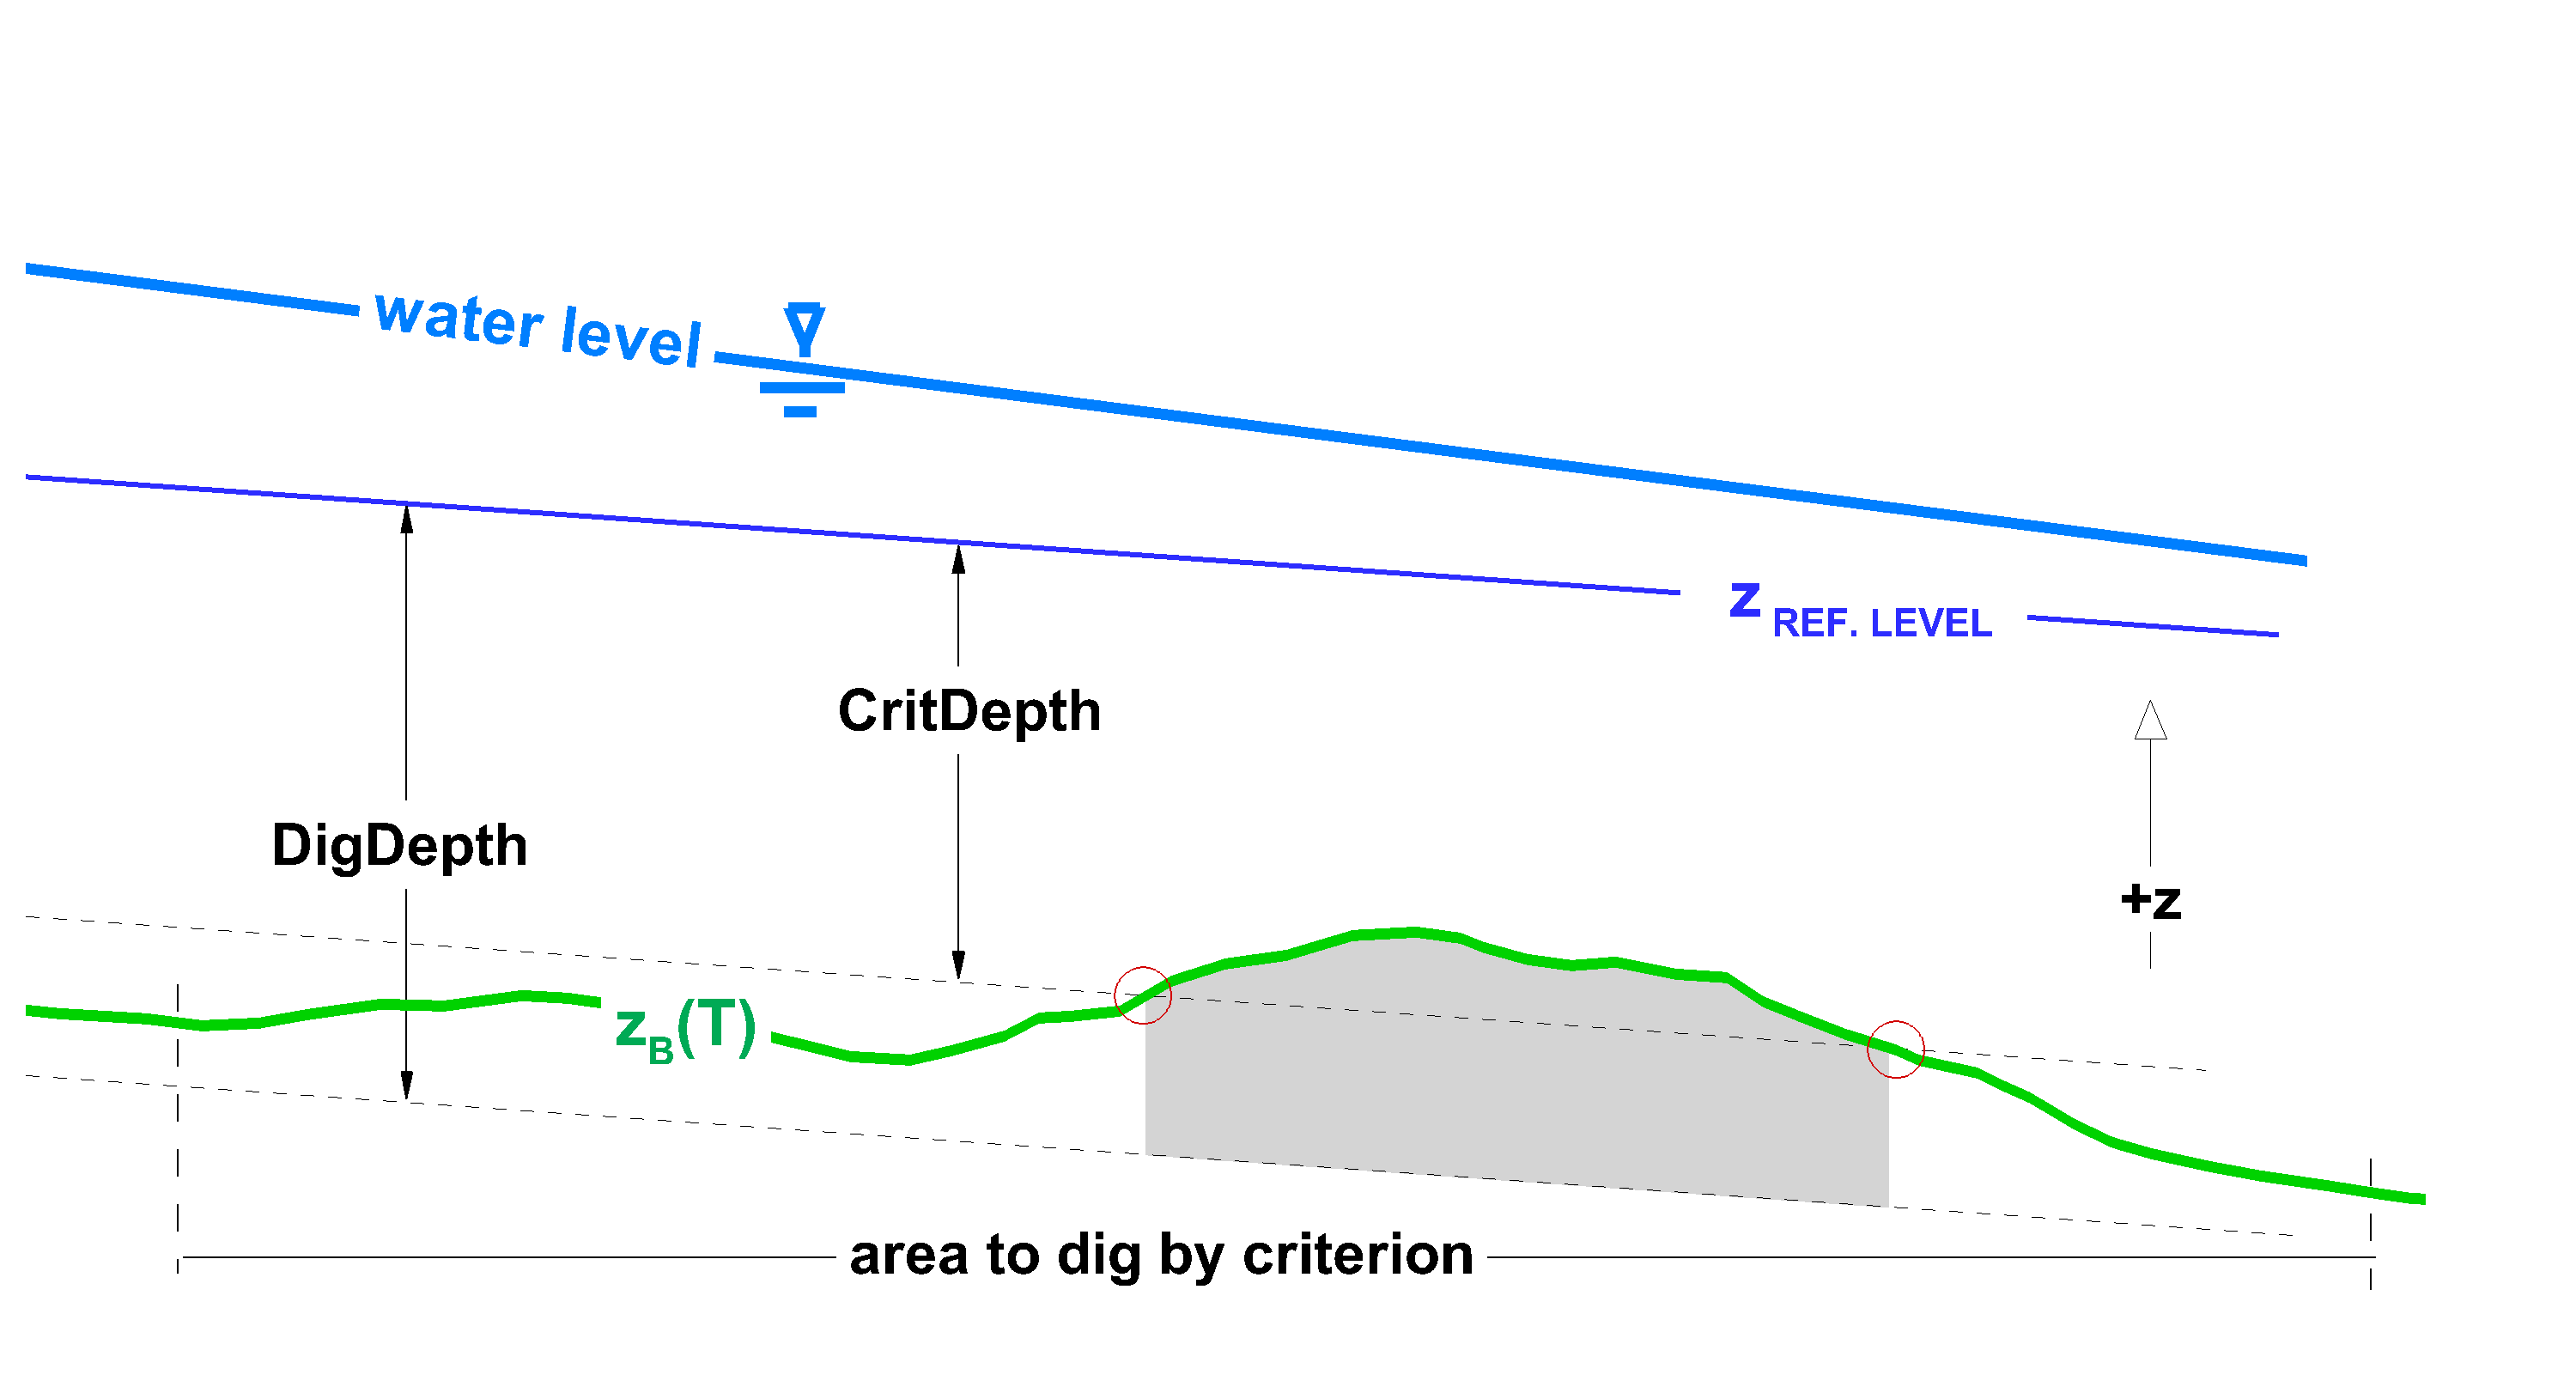
\includegraphics[scale=0.12]{critDig_schematicDiagram.png}
	\caption{Schematic diagram of dredging by criterion}\label{schema}
\end{figure}

The reference level is defined by 17 sections (see black lines in Figure \ref{grid}) which are defined in file \texttt{\_DigRefLev.dat}.
The fairway and the dumping area (see Figure~\ref{grid}) are defined by polygons which are defined in file \texttt{\_DigPolys.dat}.


Convention for naming polygons: The polygon name must start with an integer between 100 and 999. Any text after that is treated as a comment to  help the user.
Internally only the number is used to identify the polygon.




% - Physical parameters:
%     This part specifies the geometry, details all the physical parameters
%     used to describe both porous media (soil model in particularly) and
%     solute characteristics (dispersion/diffusion coefficients, soil <=> pollutant interactions...)
%
%
\subsection{Physical parameters}
%
The simulation is set up with 1 grain class.
The rigid bed is 3.0m below the initial (flat) bottom.

The Meyer-Peter Mueller (MPM) transport formula is used with the default MPM parameter. Thus all bottom changes are a result of sediment transport processes and fairway maintenance (digging and dumping).
% - Geometry and Mesh:
%     This part describes the mesh used in the computation
%
%
\subsection{Geometry and Mesh}
%
A 3.3 km long flume with two 180 degree bends has been chosen as test geometry.
The width of the flume is 200 m  (see Figure~\ref{grid}).

The mesh consists of 1614 nodes and 2948 elements.

\begin{figure} [!h]
\centering
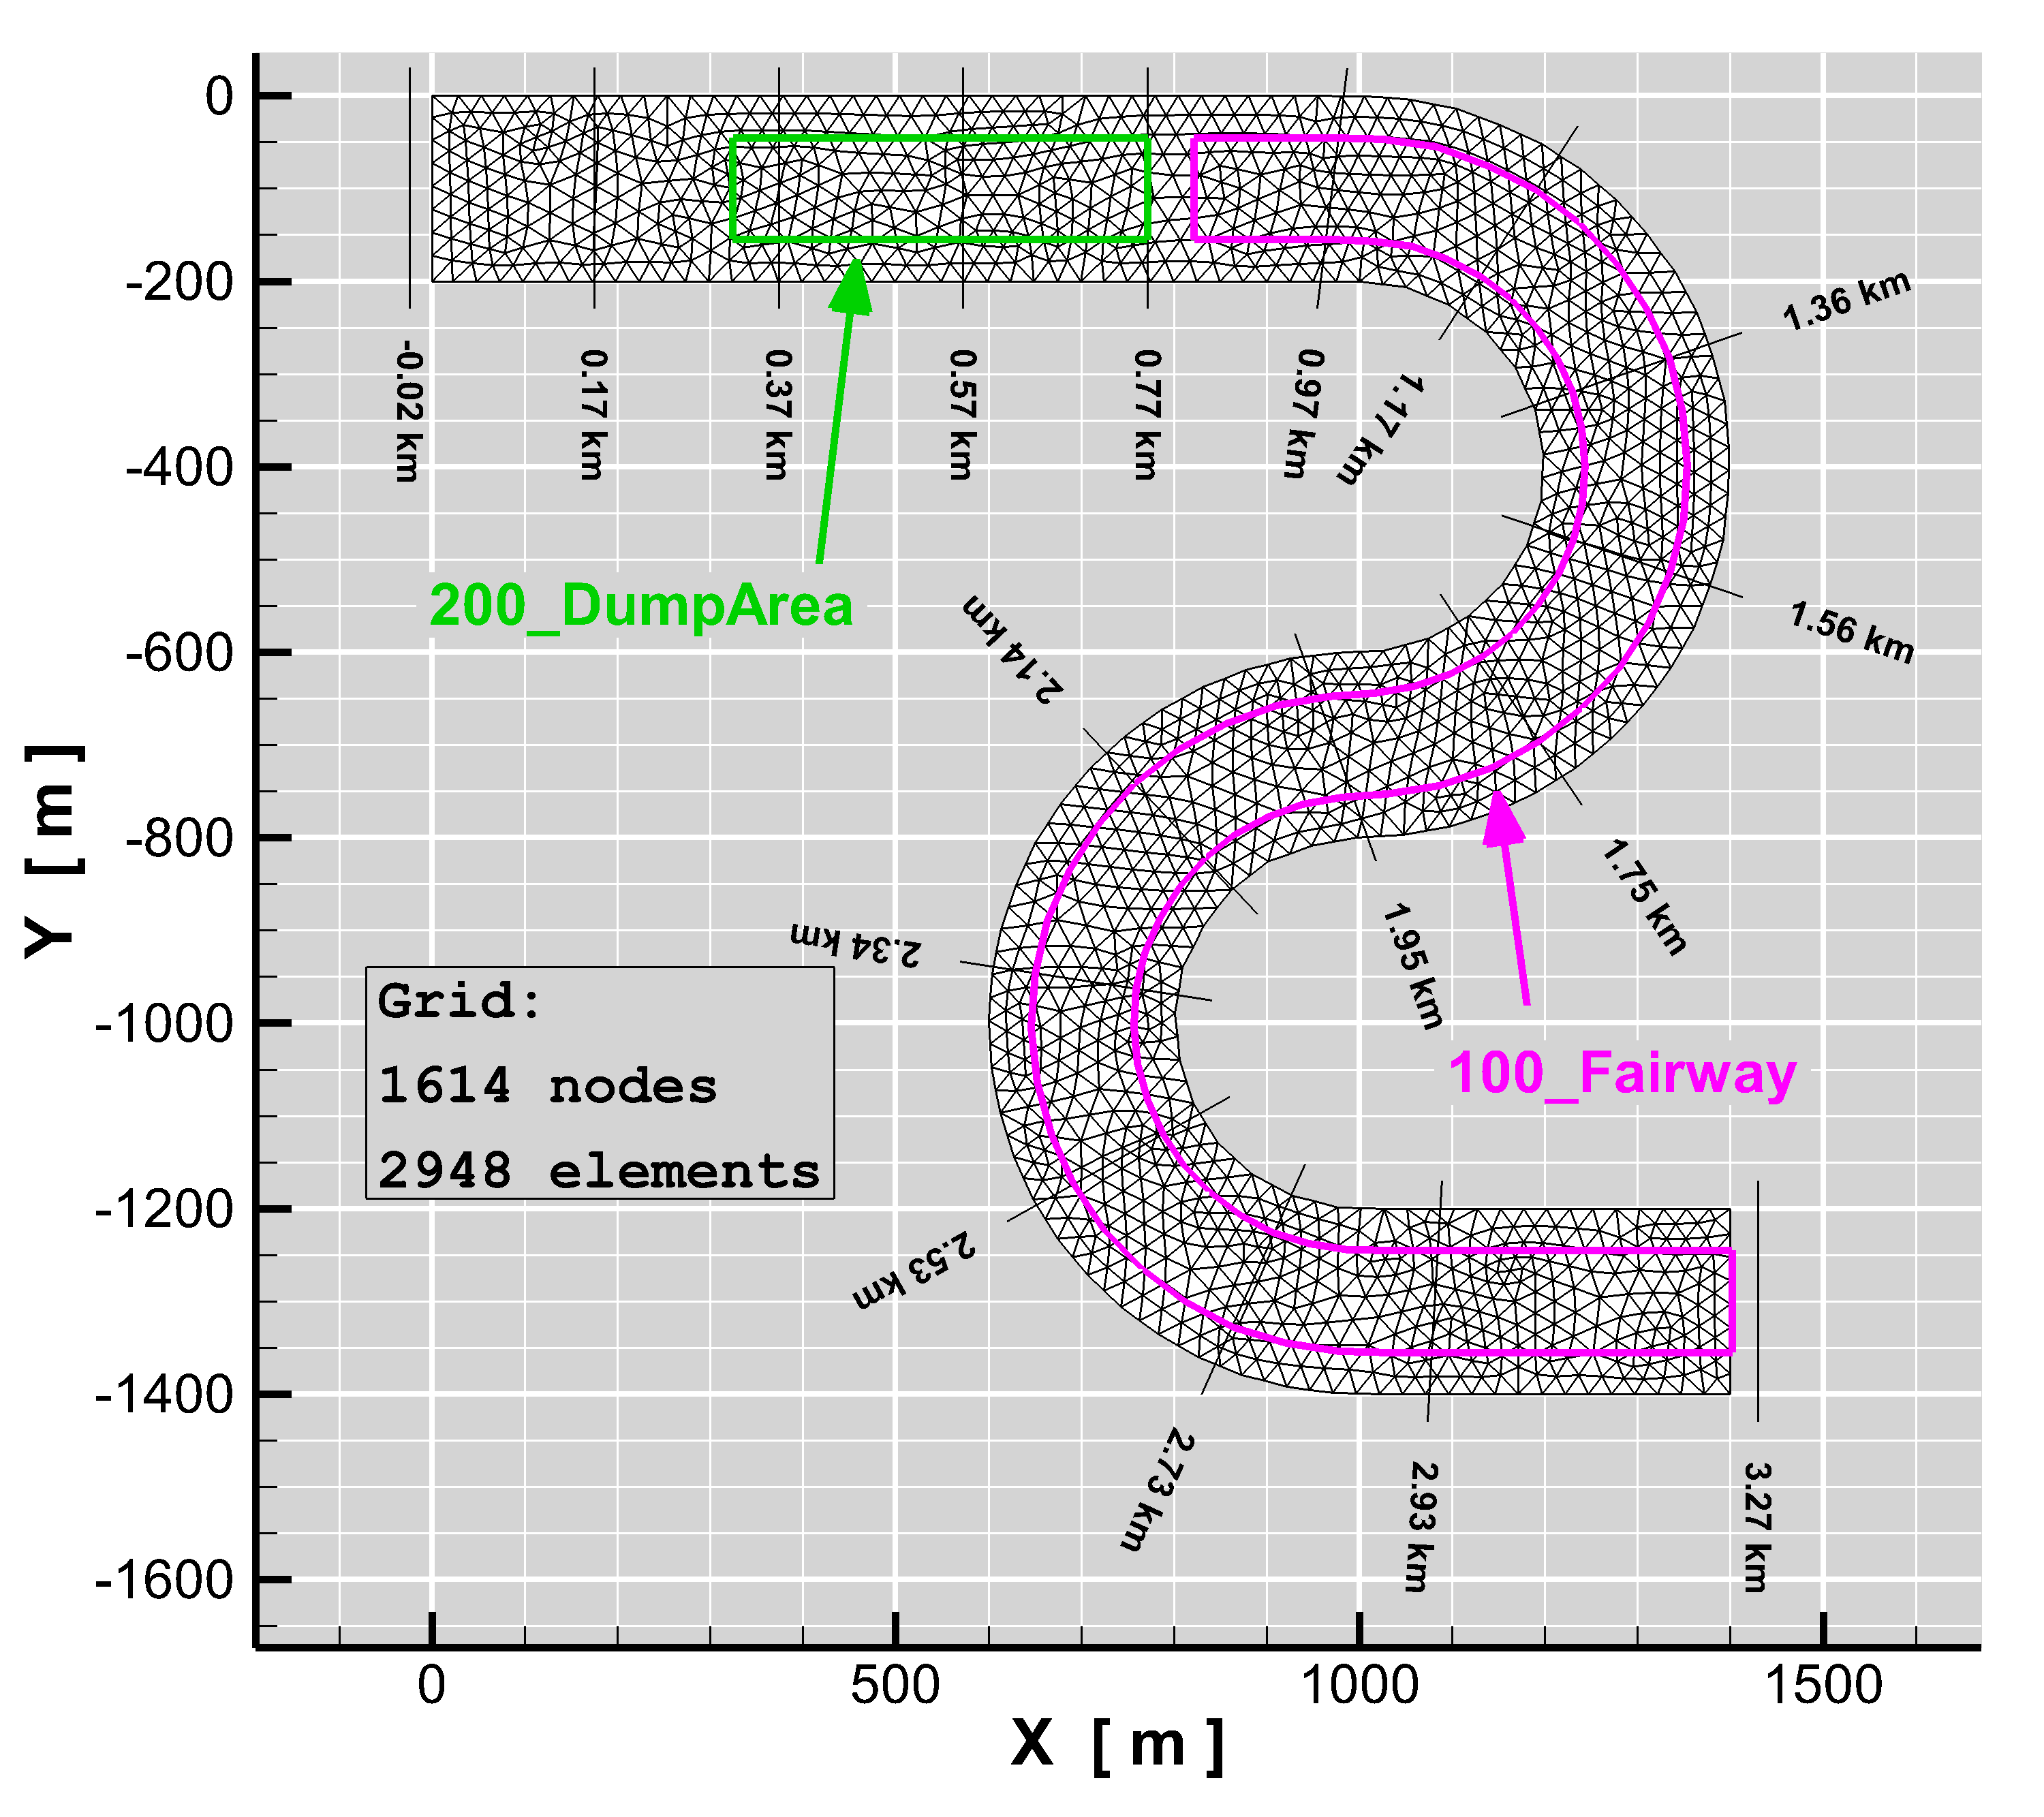
\includegraphics[scale=0.14]{critDig_grid_Polys_2D.png}
\caption{Geometry of the test flume with two bends and the two polygons (fairway, dump area) and the sections to define the reference level}\label{grid}
\end{figure}


% - Initial and boundary conditions:
%     This part details both initial and boundary conditions used to simulate the case
%
%
\subsection{Initial and Boundary Conditions}
%
Steady state boundary conditions:
\begin{itemize}
\item{Discharge at the inlet = 1000 m$^3$/s}
\item Water level at the outlet = 2.2 m
\item Sedimentological equilibrium at the inlet (zF is constant, QS is calculated)
\end{itemize}
Fully developed flow and bottom from a previous simulation are used as initial conditions.

The simulation period is 1200000.0 s (13.88 days) with a time step of 4 s.
% - Numerical parameters:
%     This part is used to specify the numerical parameters used
%     (adaptive time step, mass-lumping when necessary...)
%
%
\subsection{Numerical parameters}
%
% - Results:
%     We comment in this part the numerical results against the reference ones,
%     giving understanding keys and making assumptions when necessary.
%
%
\section{Results}
%
Figure \ref{result12} shows the bottom evolution after 0h and 1h. The evolution after 0d is from a previous computation file. The evolution after 1d is driven by the first maintenance of the fairway and sediment transport. The digging and dumping were executed between 0d and 1d. The fairway was dredged to the \texttt{DigDepth} and the dredged material was dumped to the dumping area defined by the polygon \texttt{200\_DumpArea}.



Figure \ref{result34} and \ref{result56} shows the bottom evolution due to sediment transport processes after 3d, 7d and 10d.
No digging and dumping actions were defined in this time period. Between 10d and 11d the second maintenance was executed. Again the fairway was dredged to the
\texttt{DigDepth} and the dredged material was dumped to the dumping area, which leaded again to a higher bottom evolution.

Figure \ref{result78} shows the bottom evolution  12d and 13.5d due to sediment transport processes after the second maintenance of the fairway.

% Here is an example of how to include the graph generated by validateTELEMAC.py
% They should be in test_case/img
\begin{figure} [!h]
\centering
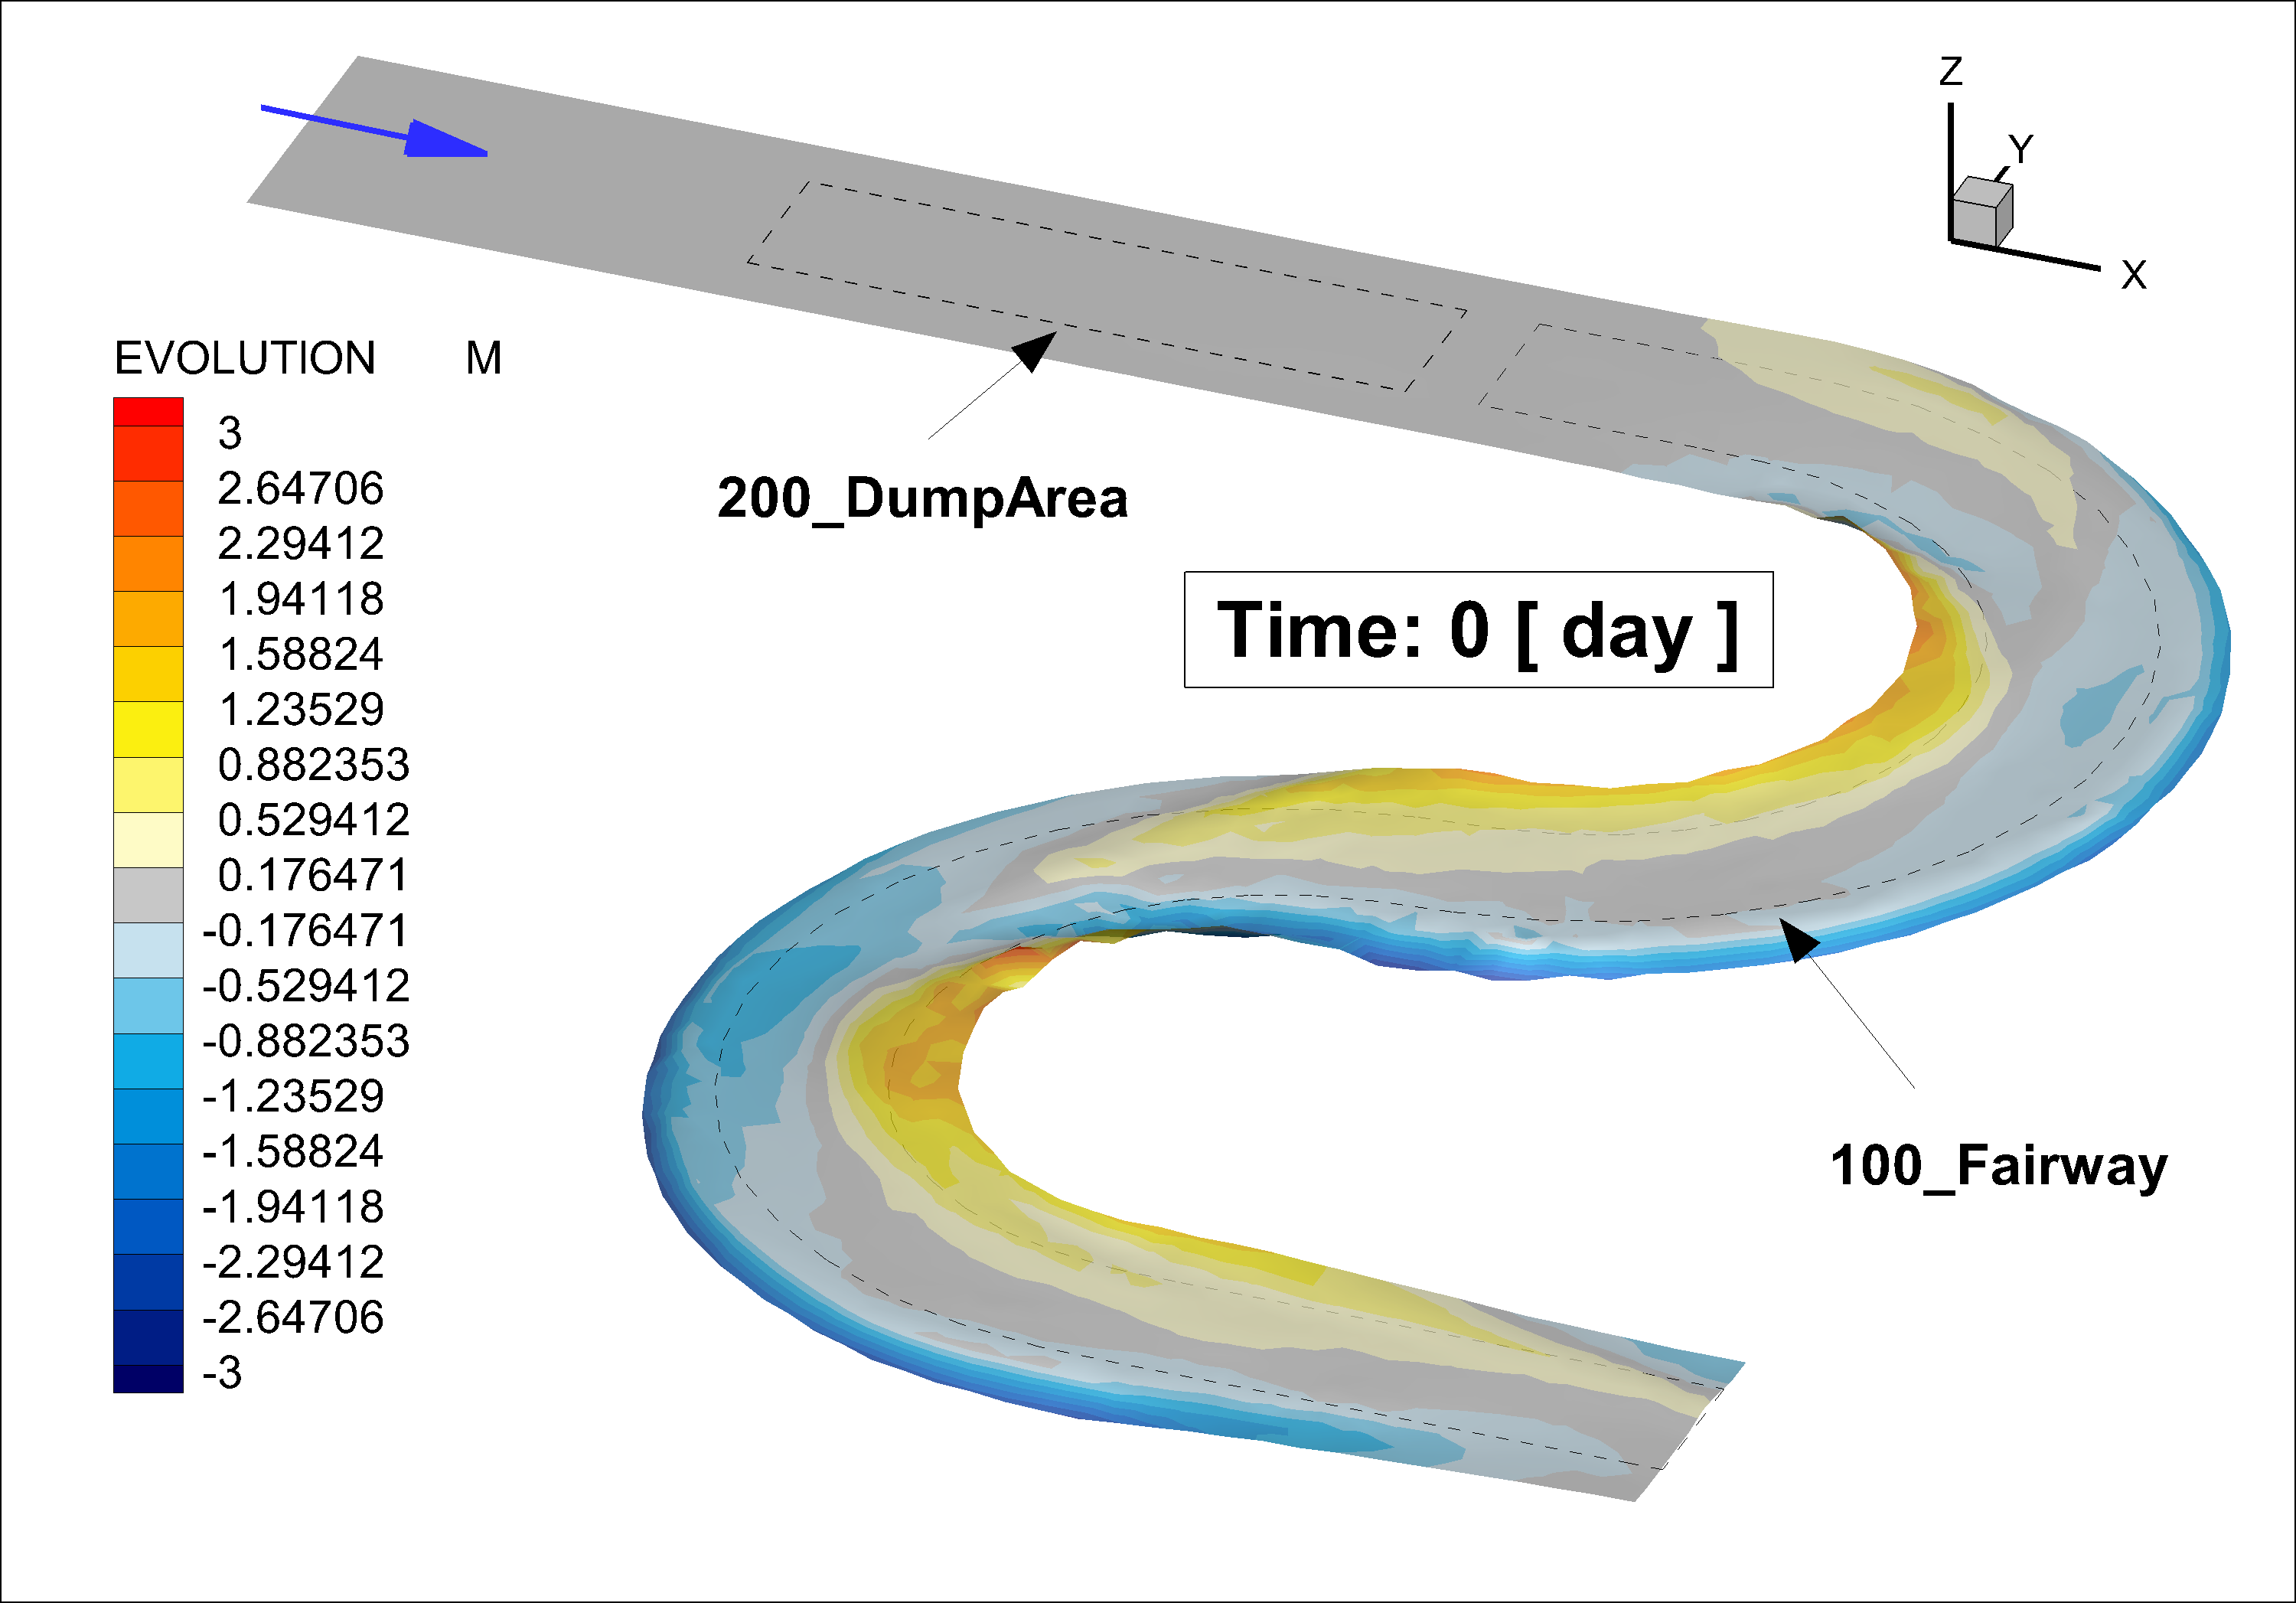
\includegraphics[scale=0.14]{critDig_Poly_00p0d.png}
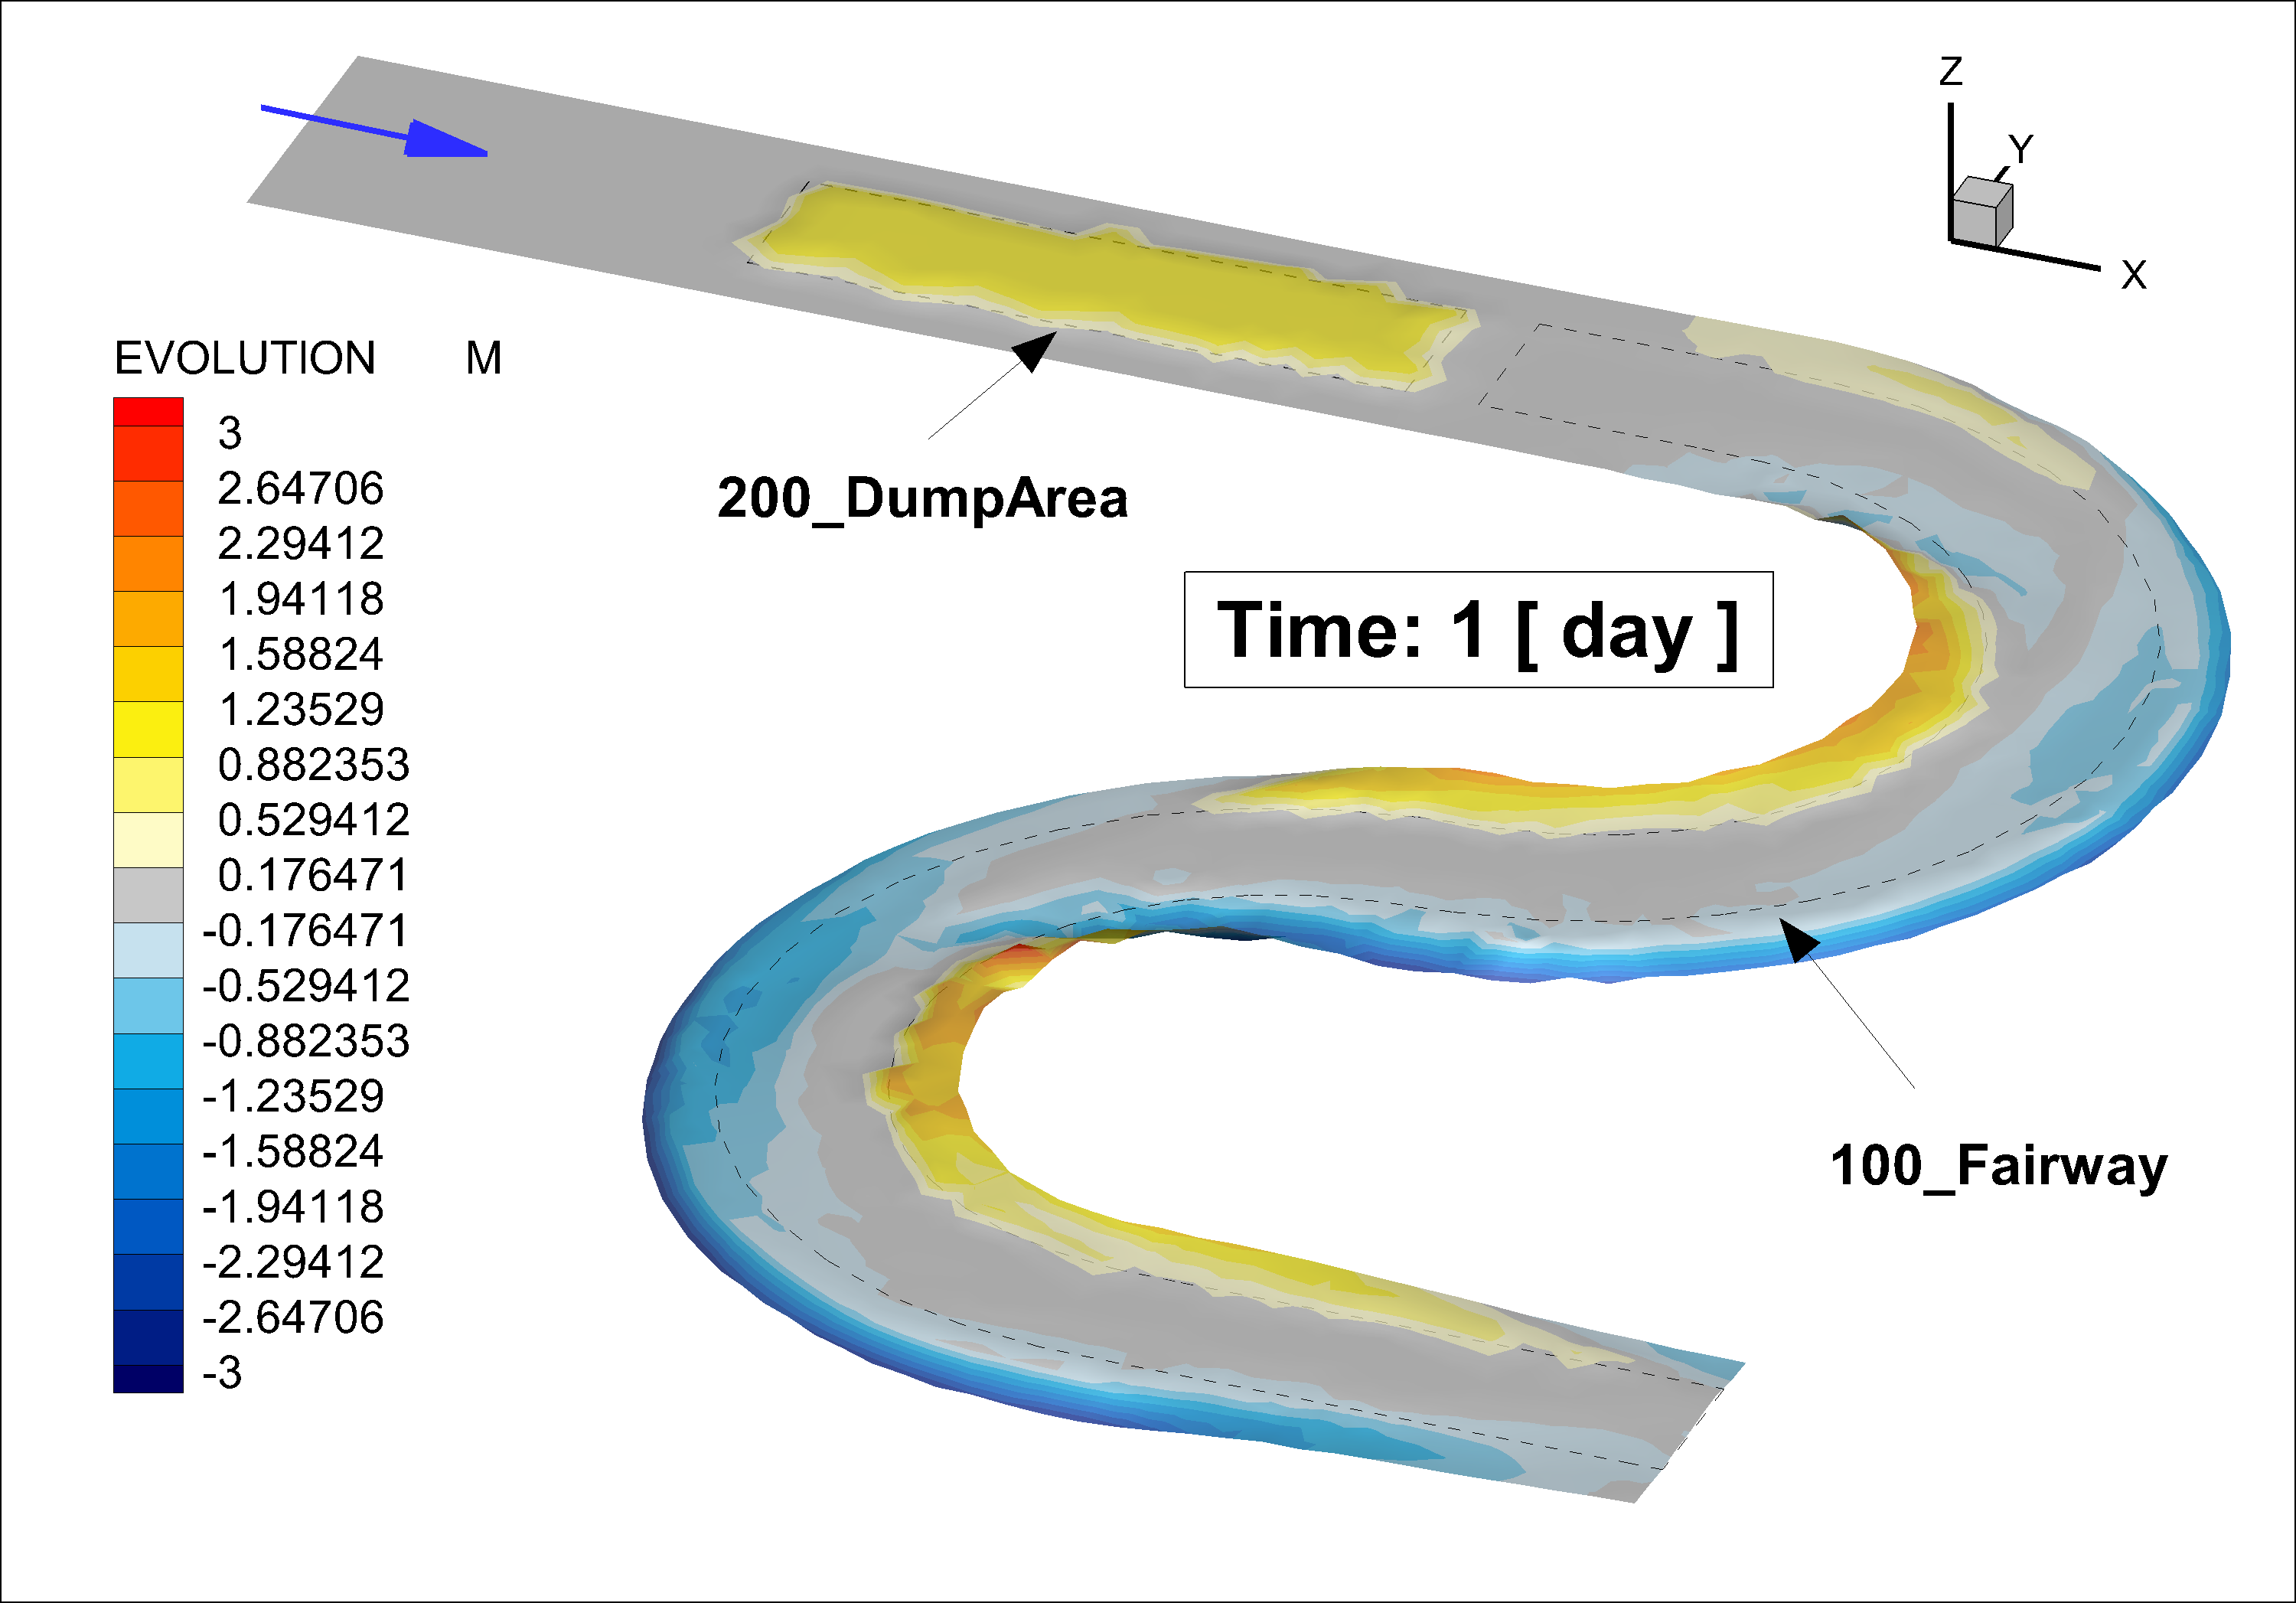
\includegraphics[scale=0.14]{critDig_Poly_01p0d.png}
\caption{Simulated evolution over the time.}\label{result12}
\end{figure}

\begin{figure} [!h]
\centering
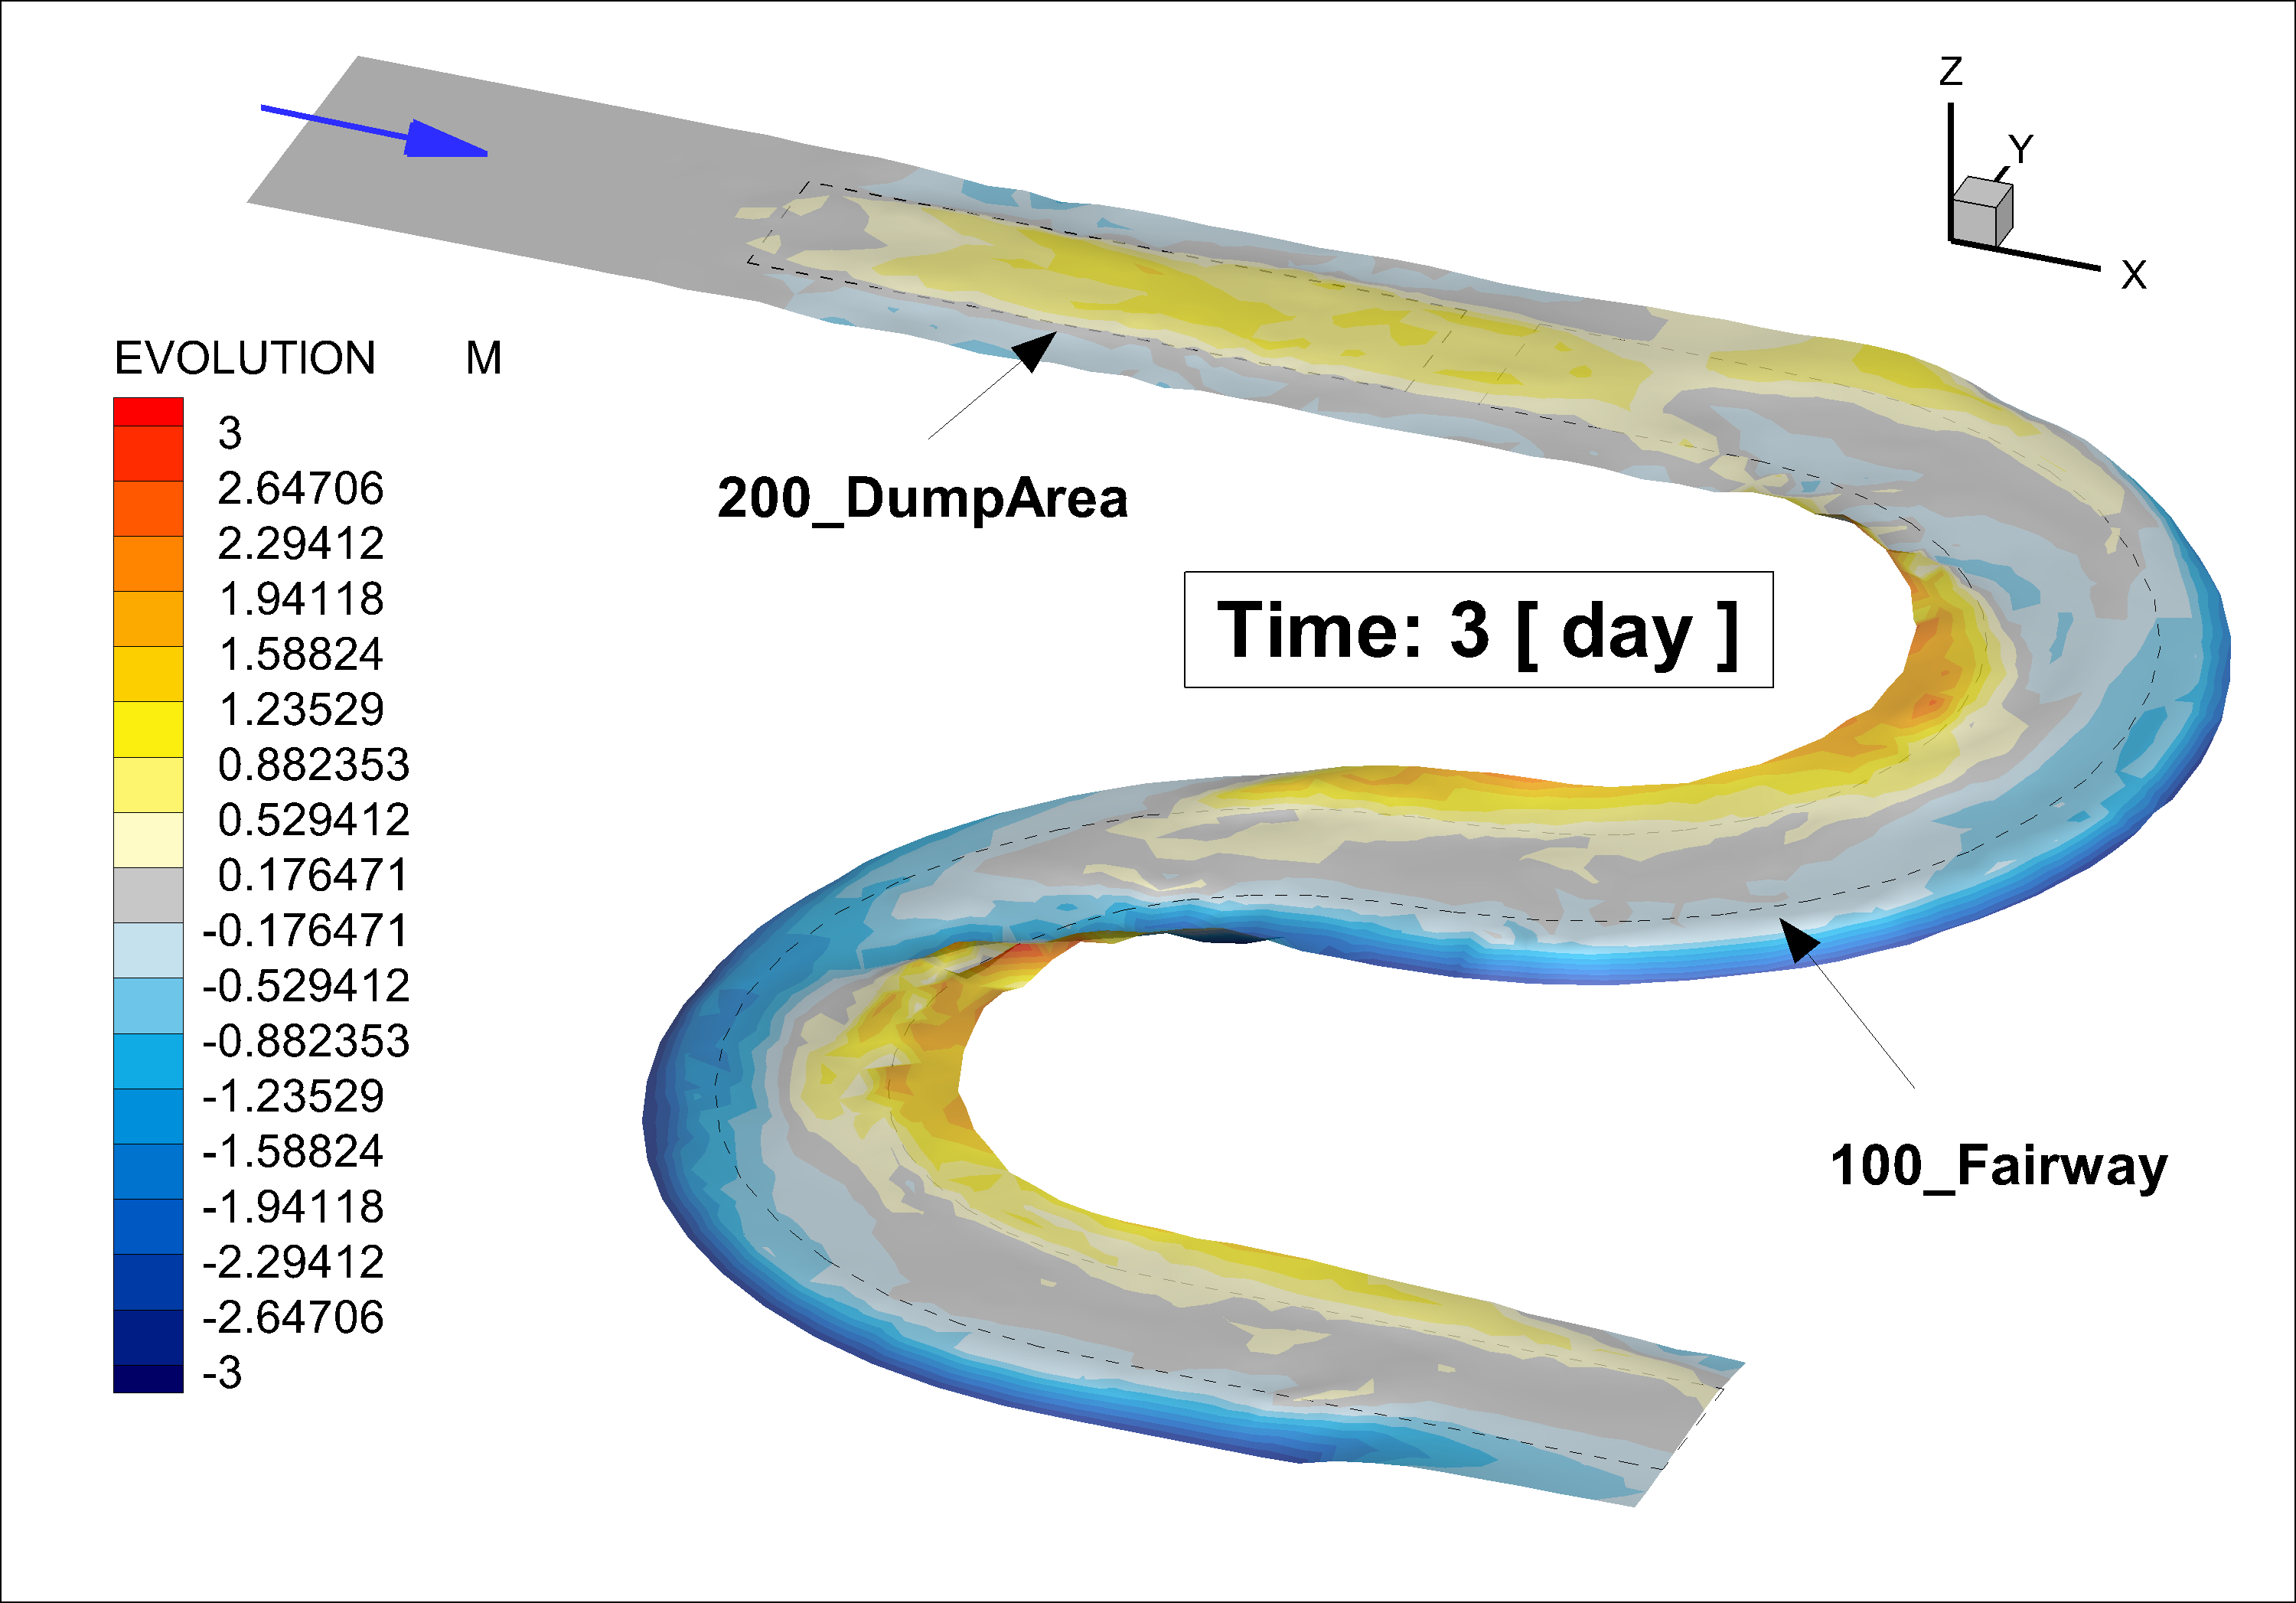
\includegraphics[scale=0.14]{critDig_Poly_03p0d.png}
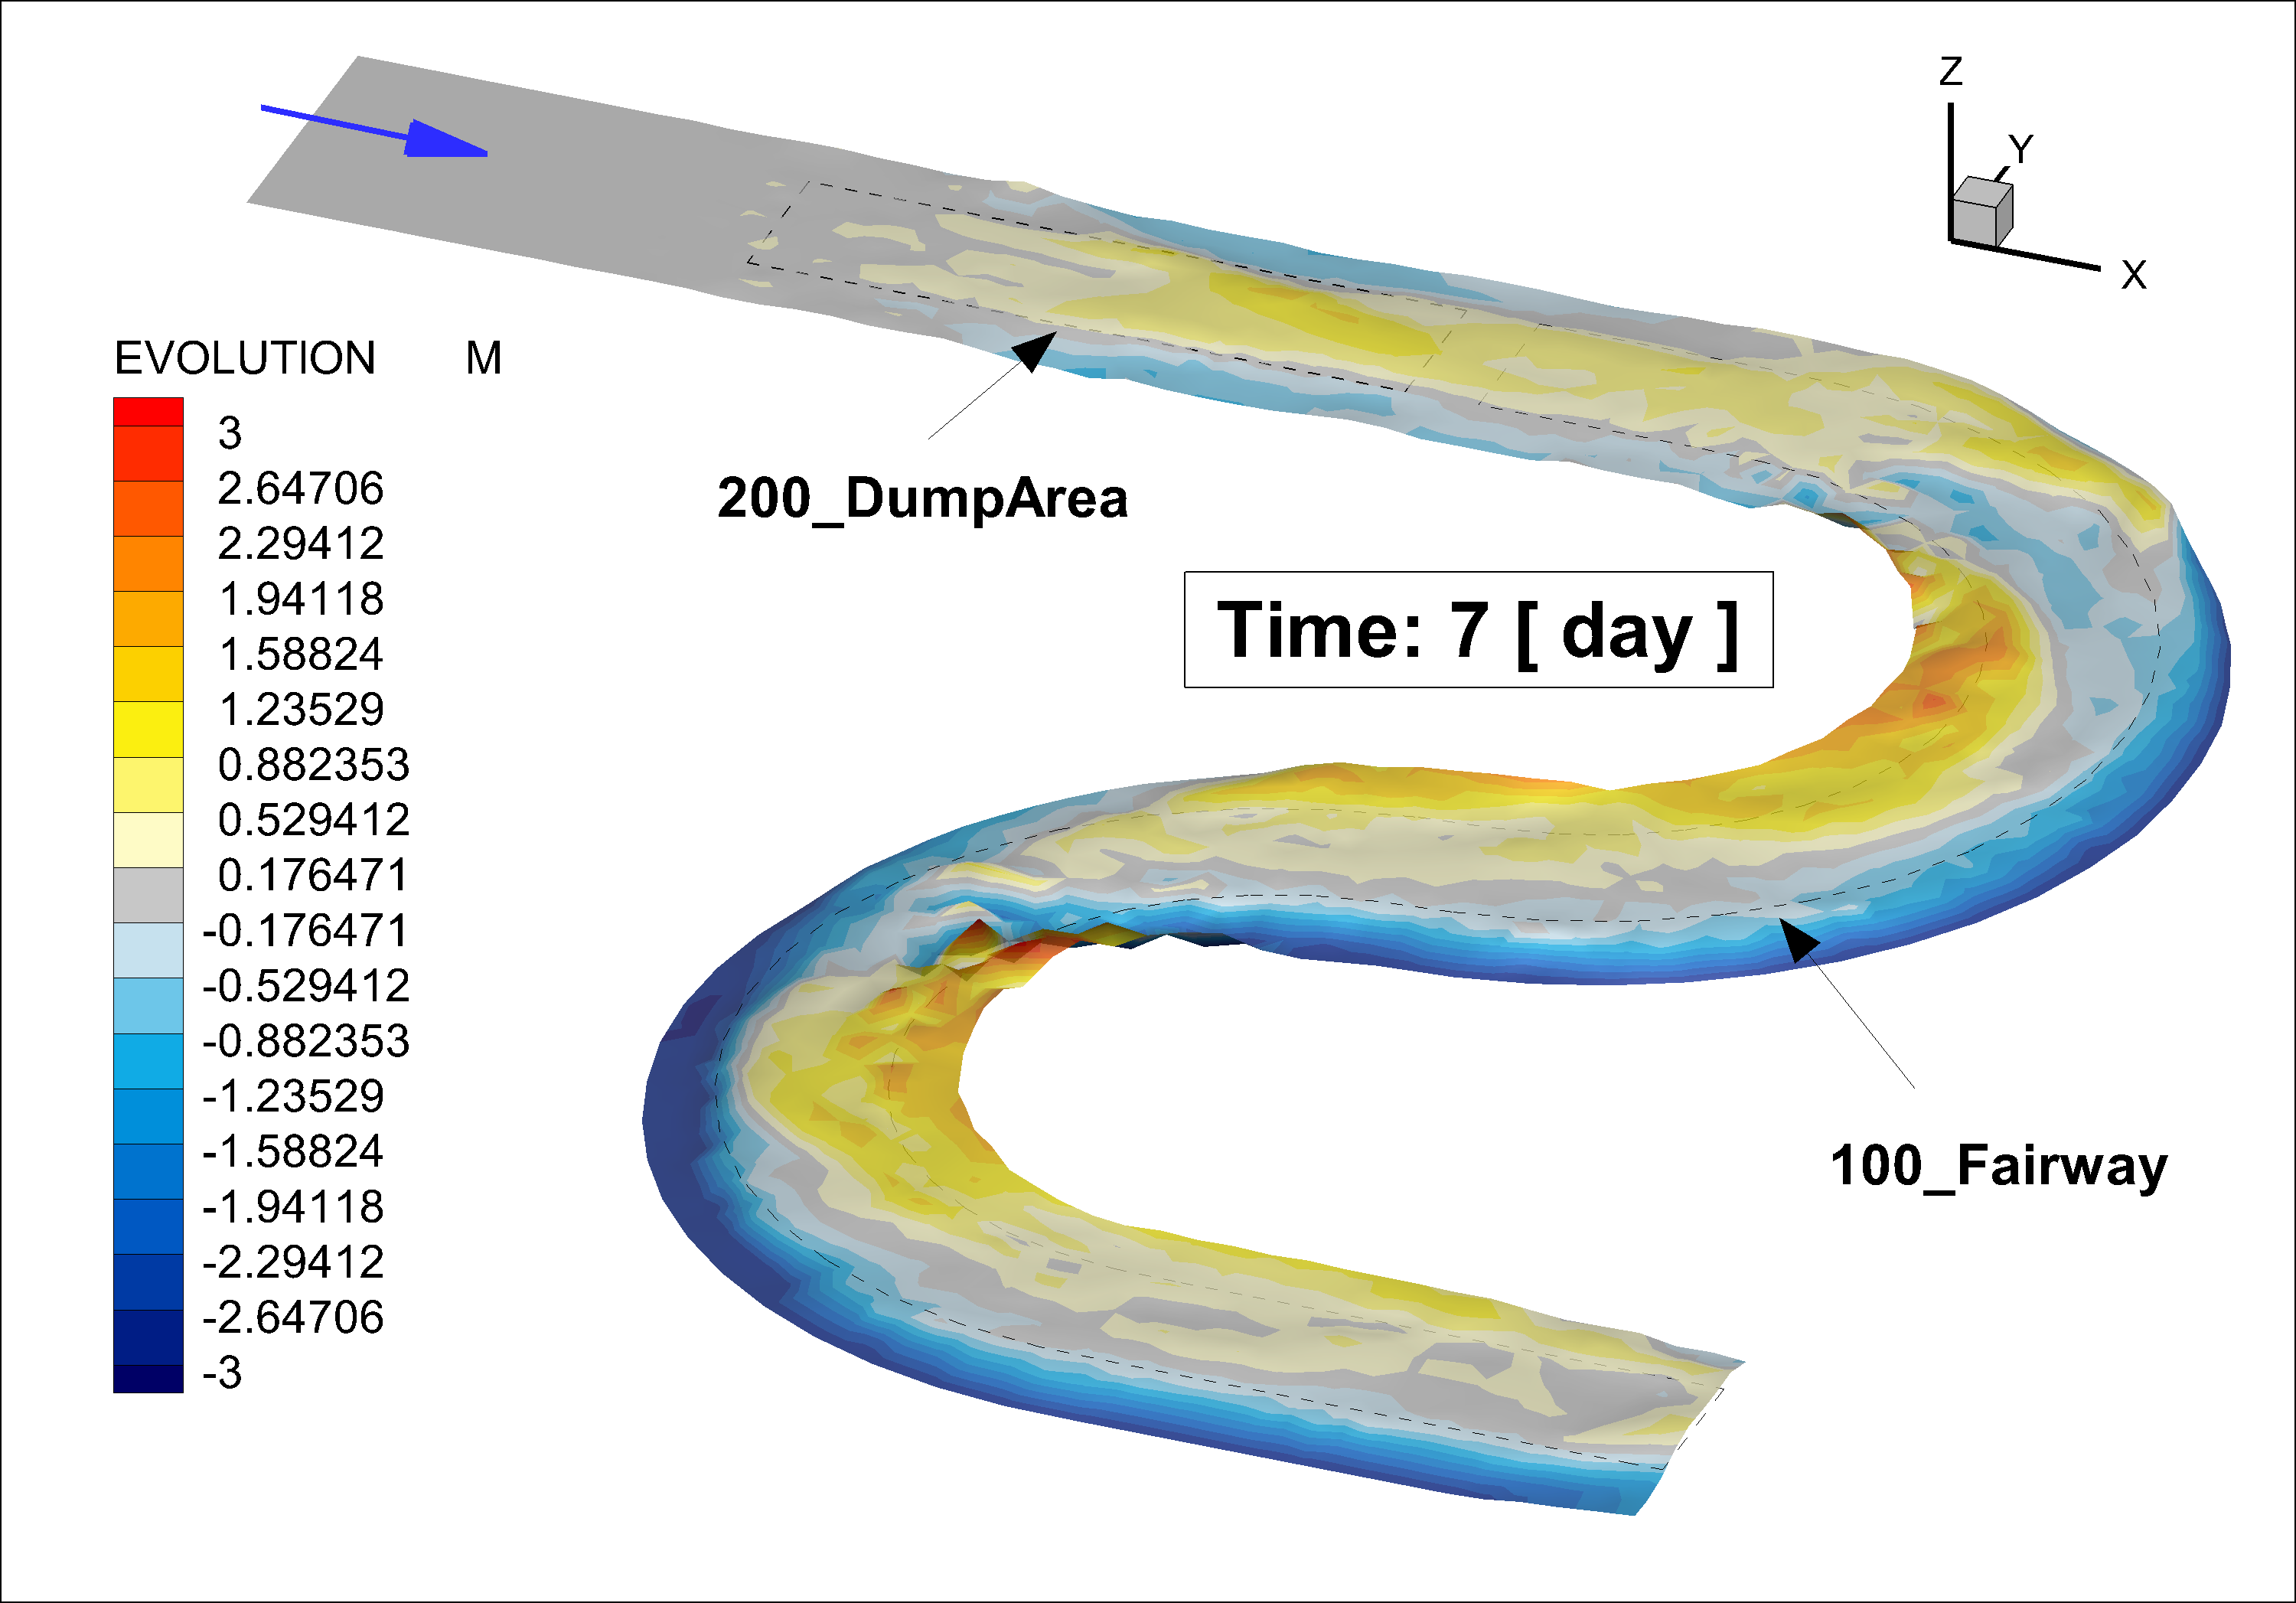
\includegraphics[scale=0.14]{critDig_Poly_07p0d.png}
\caption{Simulated evolution over the time.}\label{result34}
\end{figure}

\begin{figure} [!h]
\centering
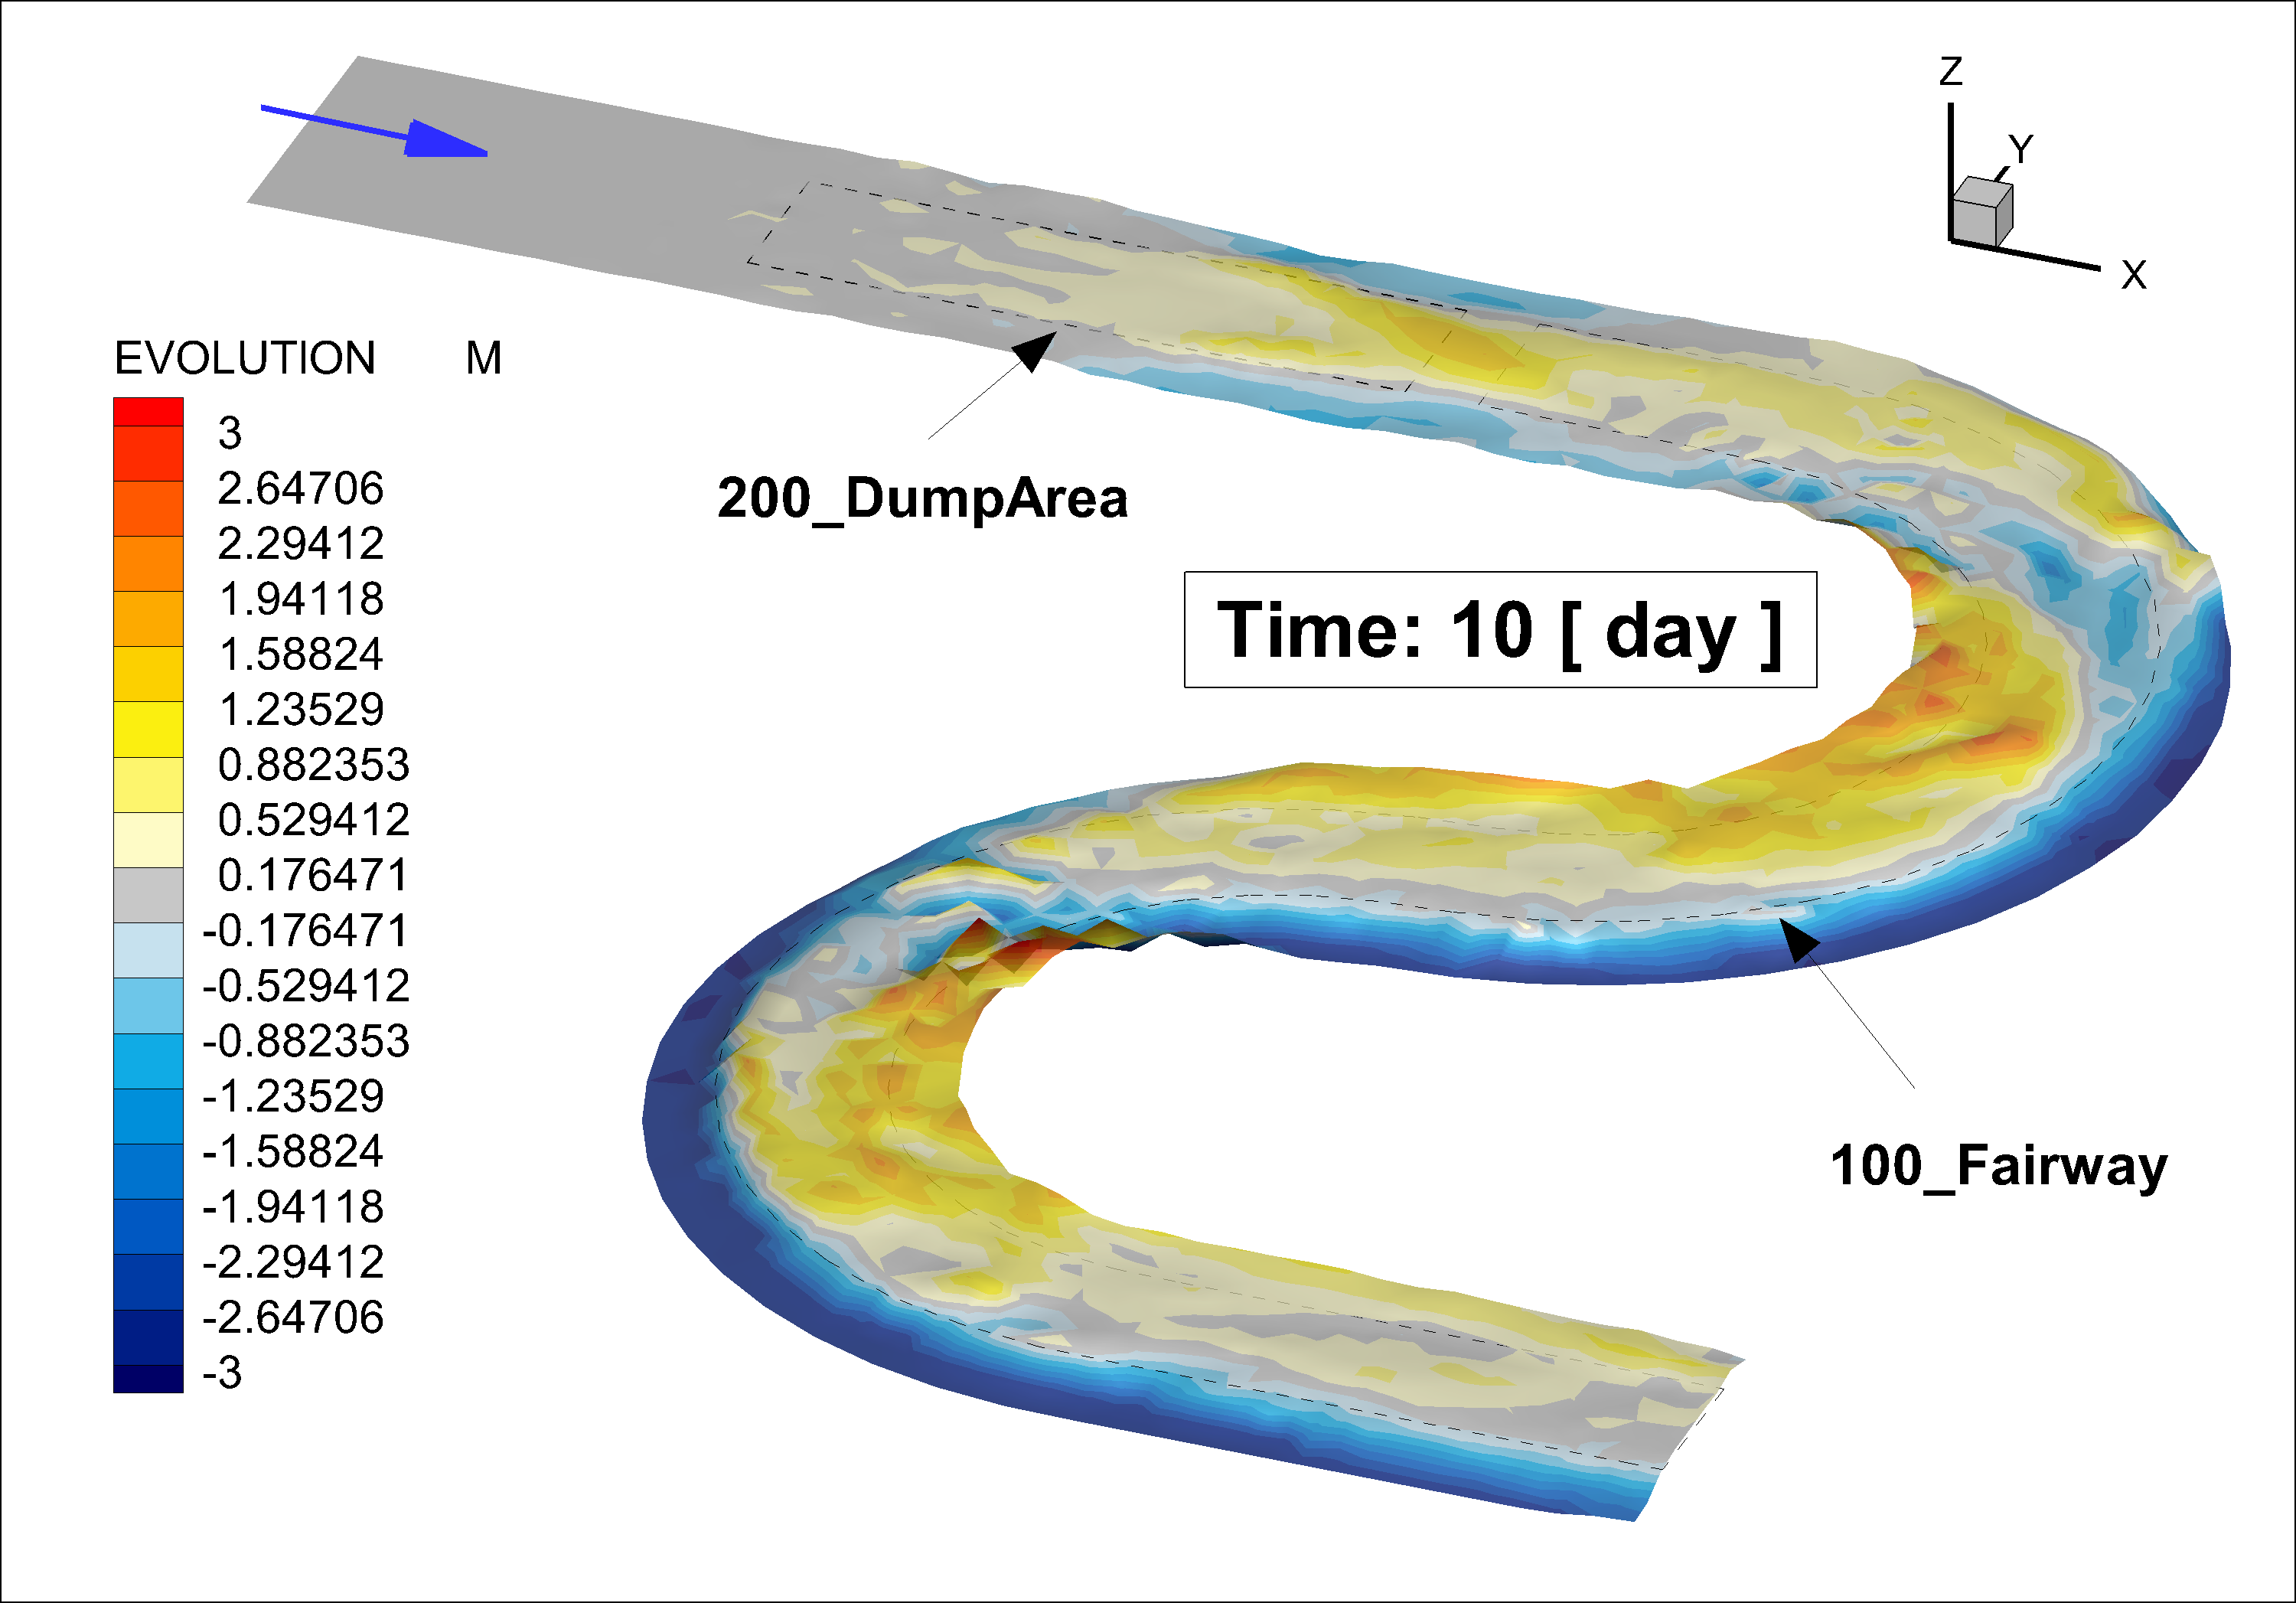
\includegraphics[scale=0.14]{critDig_Poly_10p0d.png}
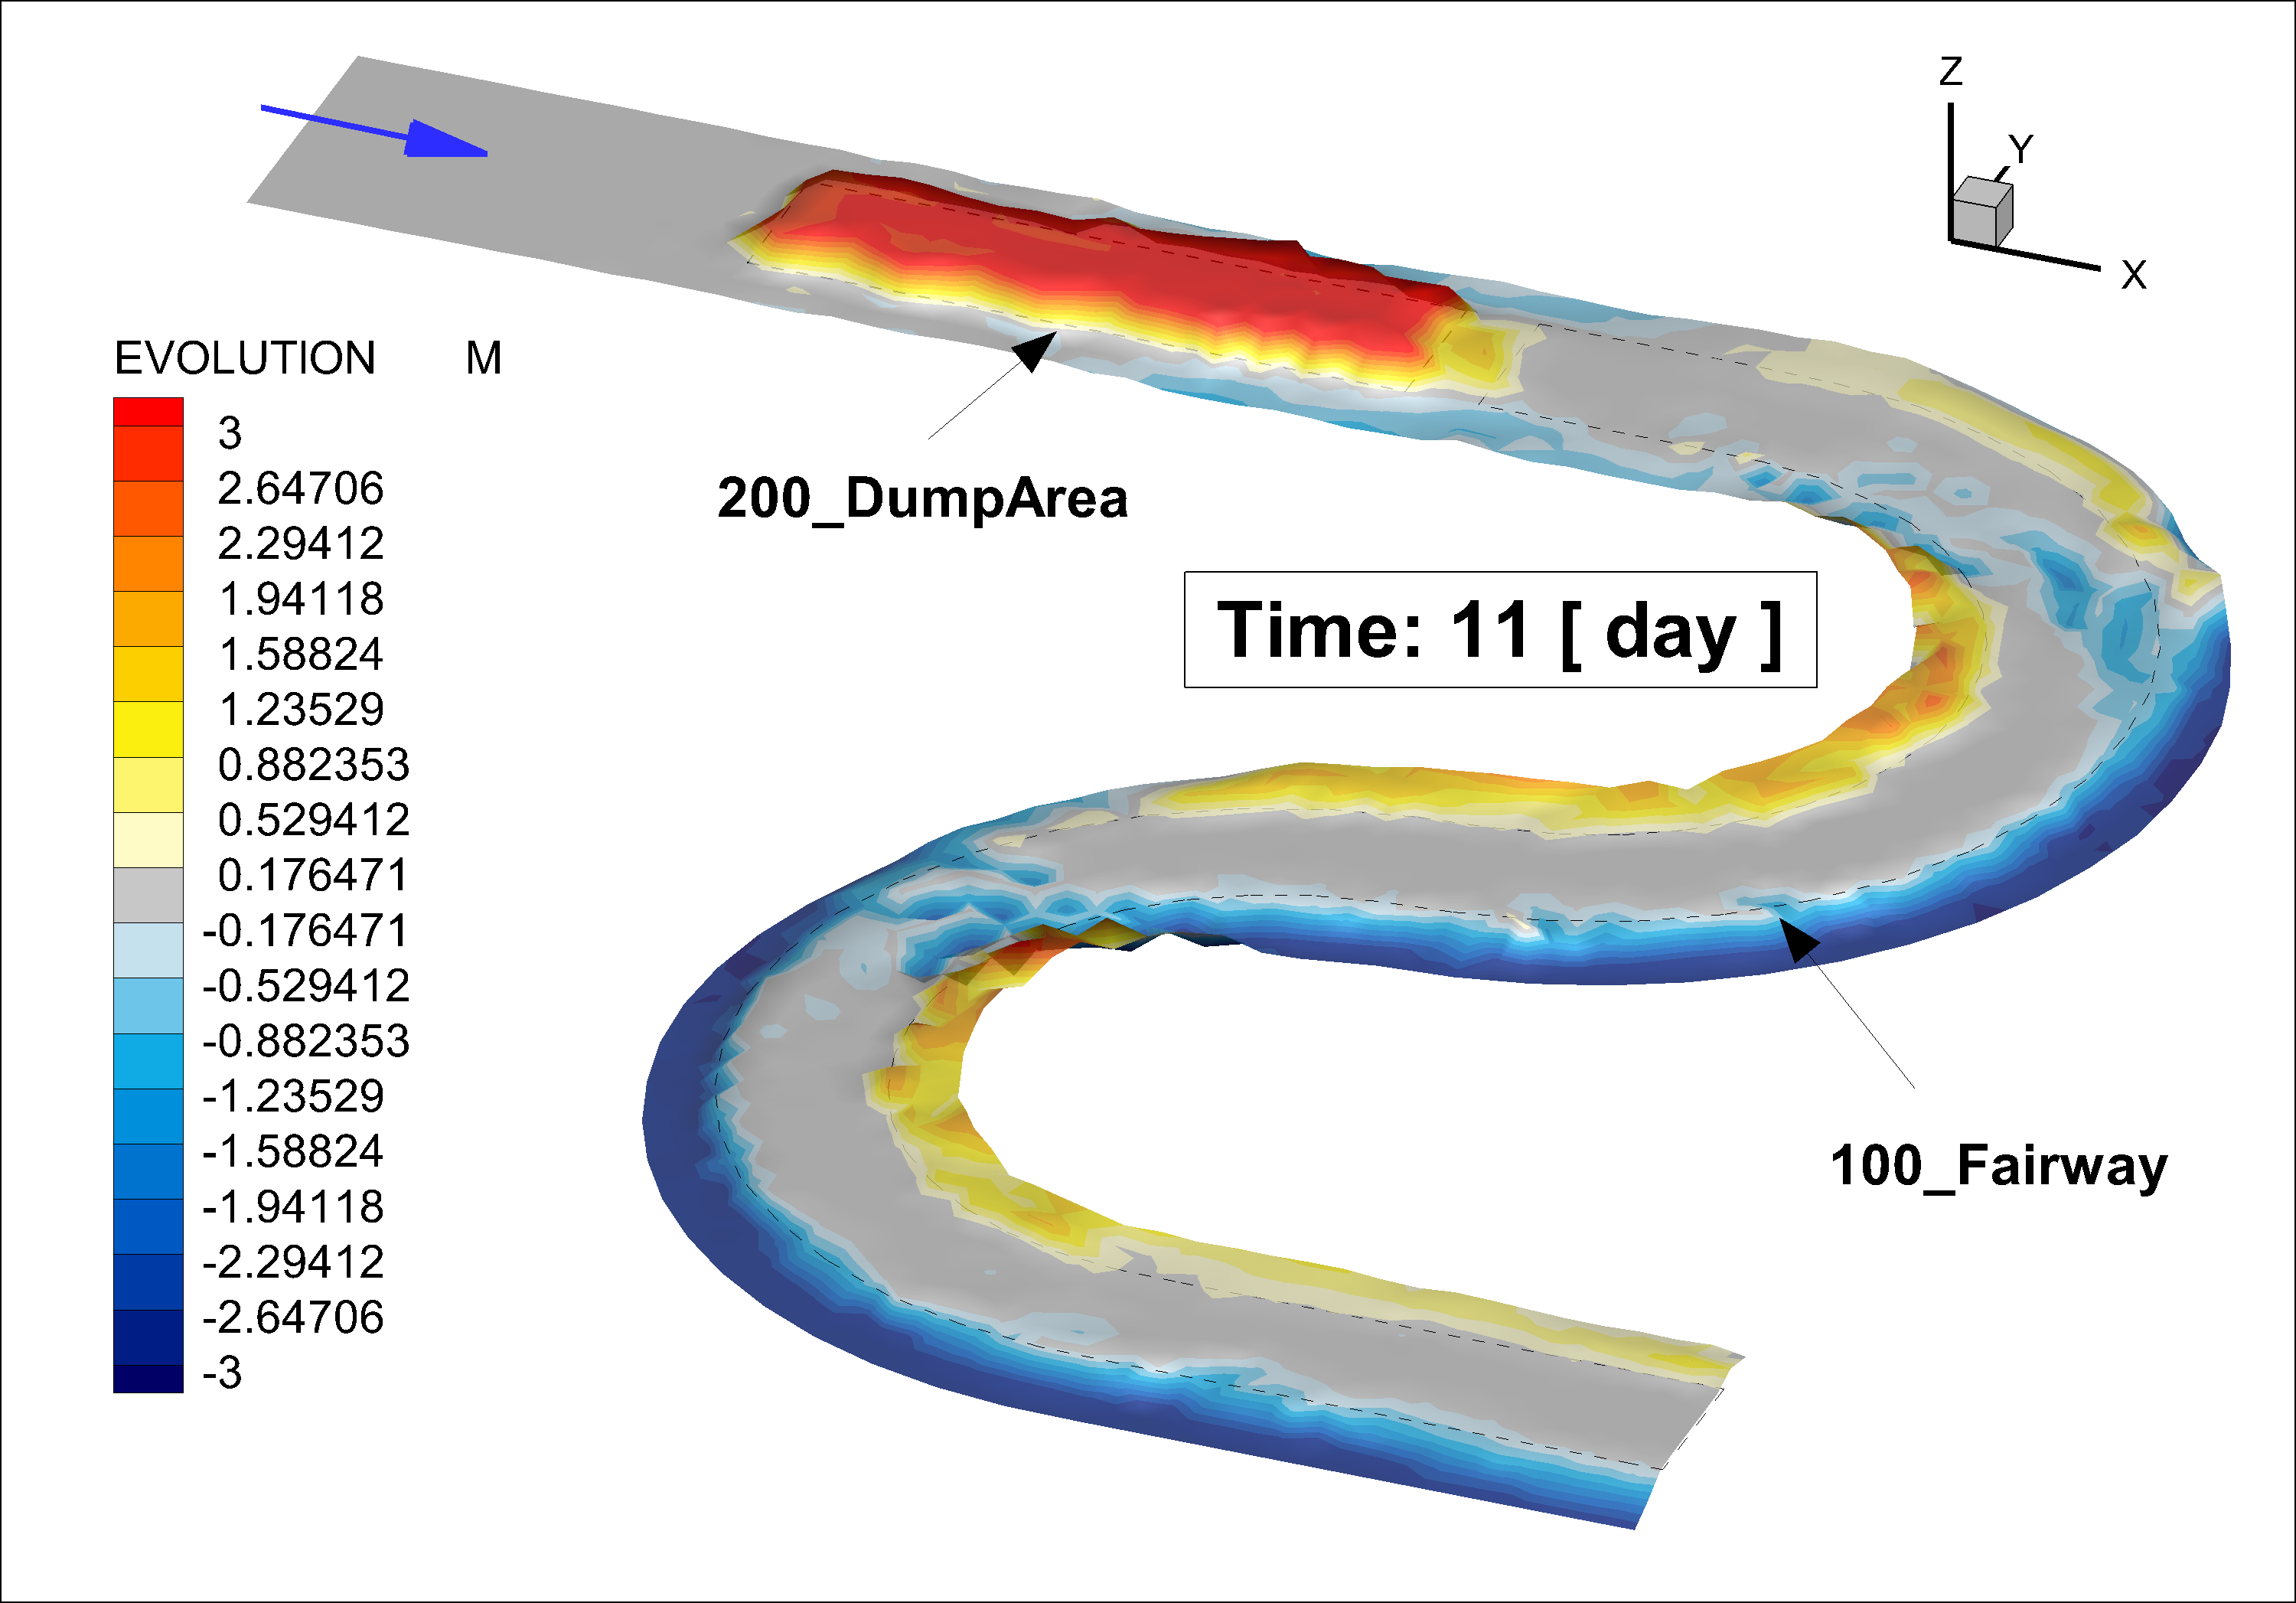
\includegraphics[scale=0.14]{critDig_Poly_11p0d.png}
\caption{Simulated evolution over the time.}\label{result56}
\end{figure}

\begin{figure} [!h]
\centering
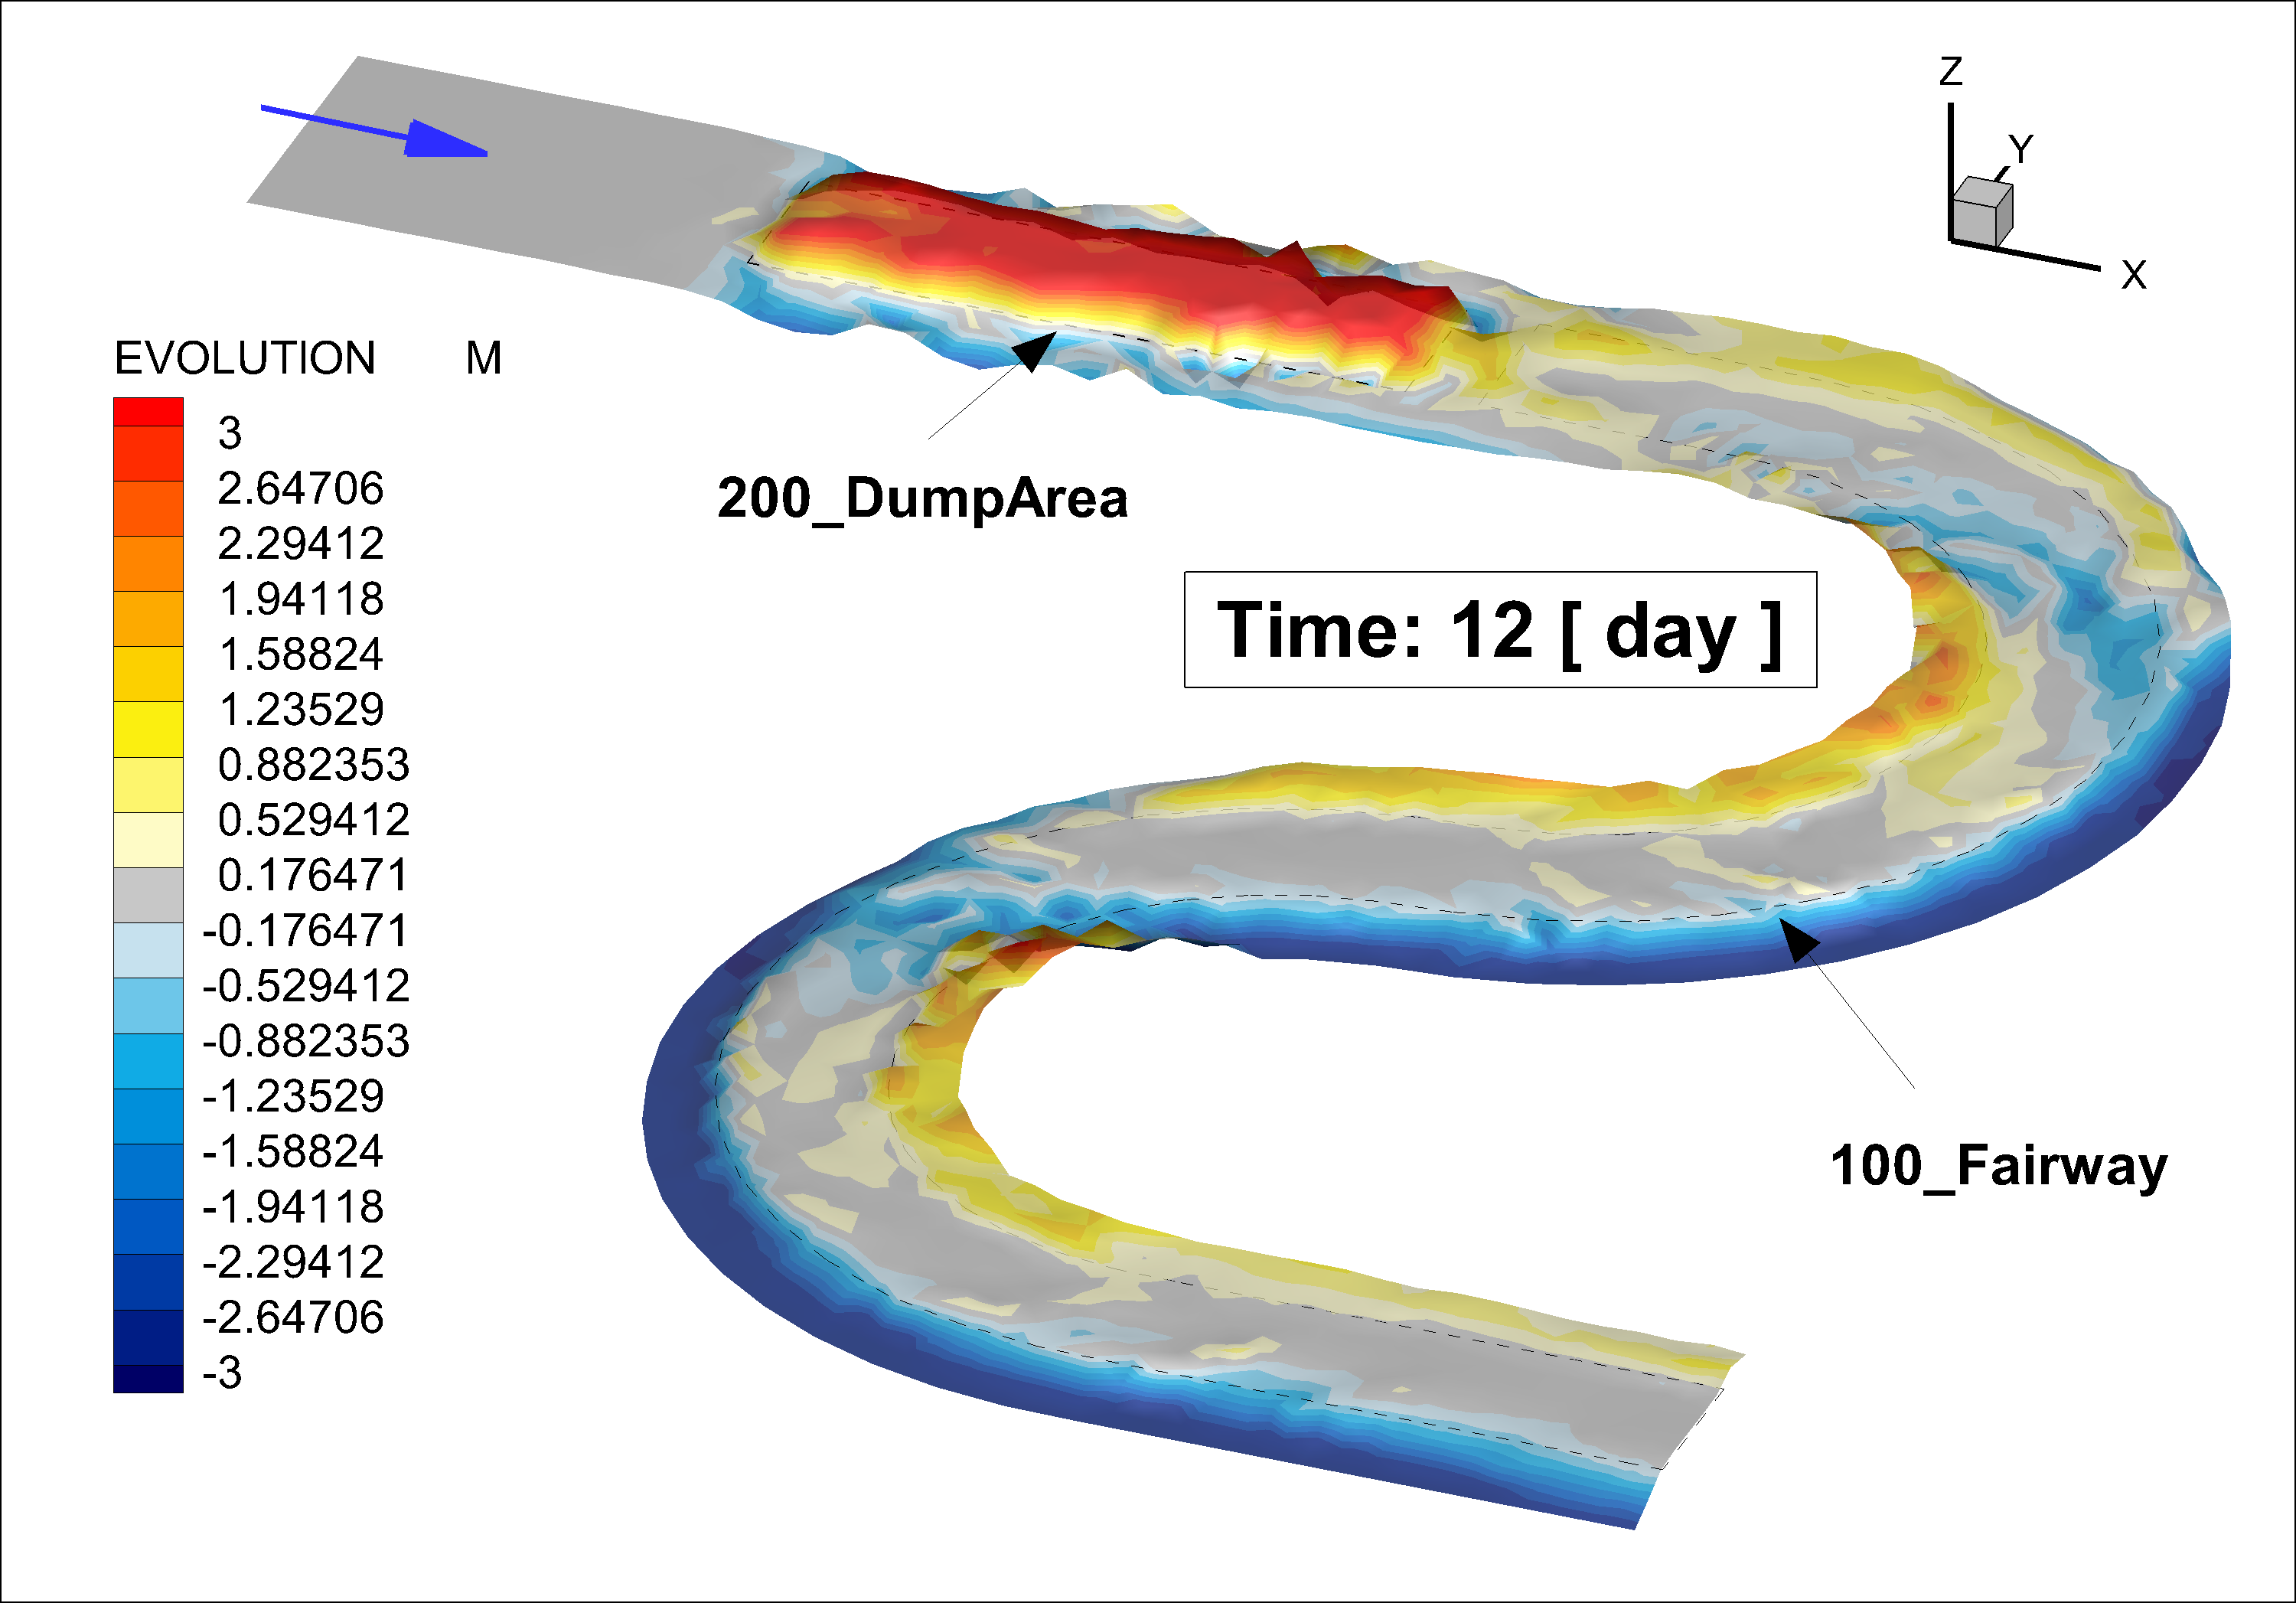
\includegraphics[scale=0.14]{critDig_Poly_12p0d.png}
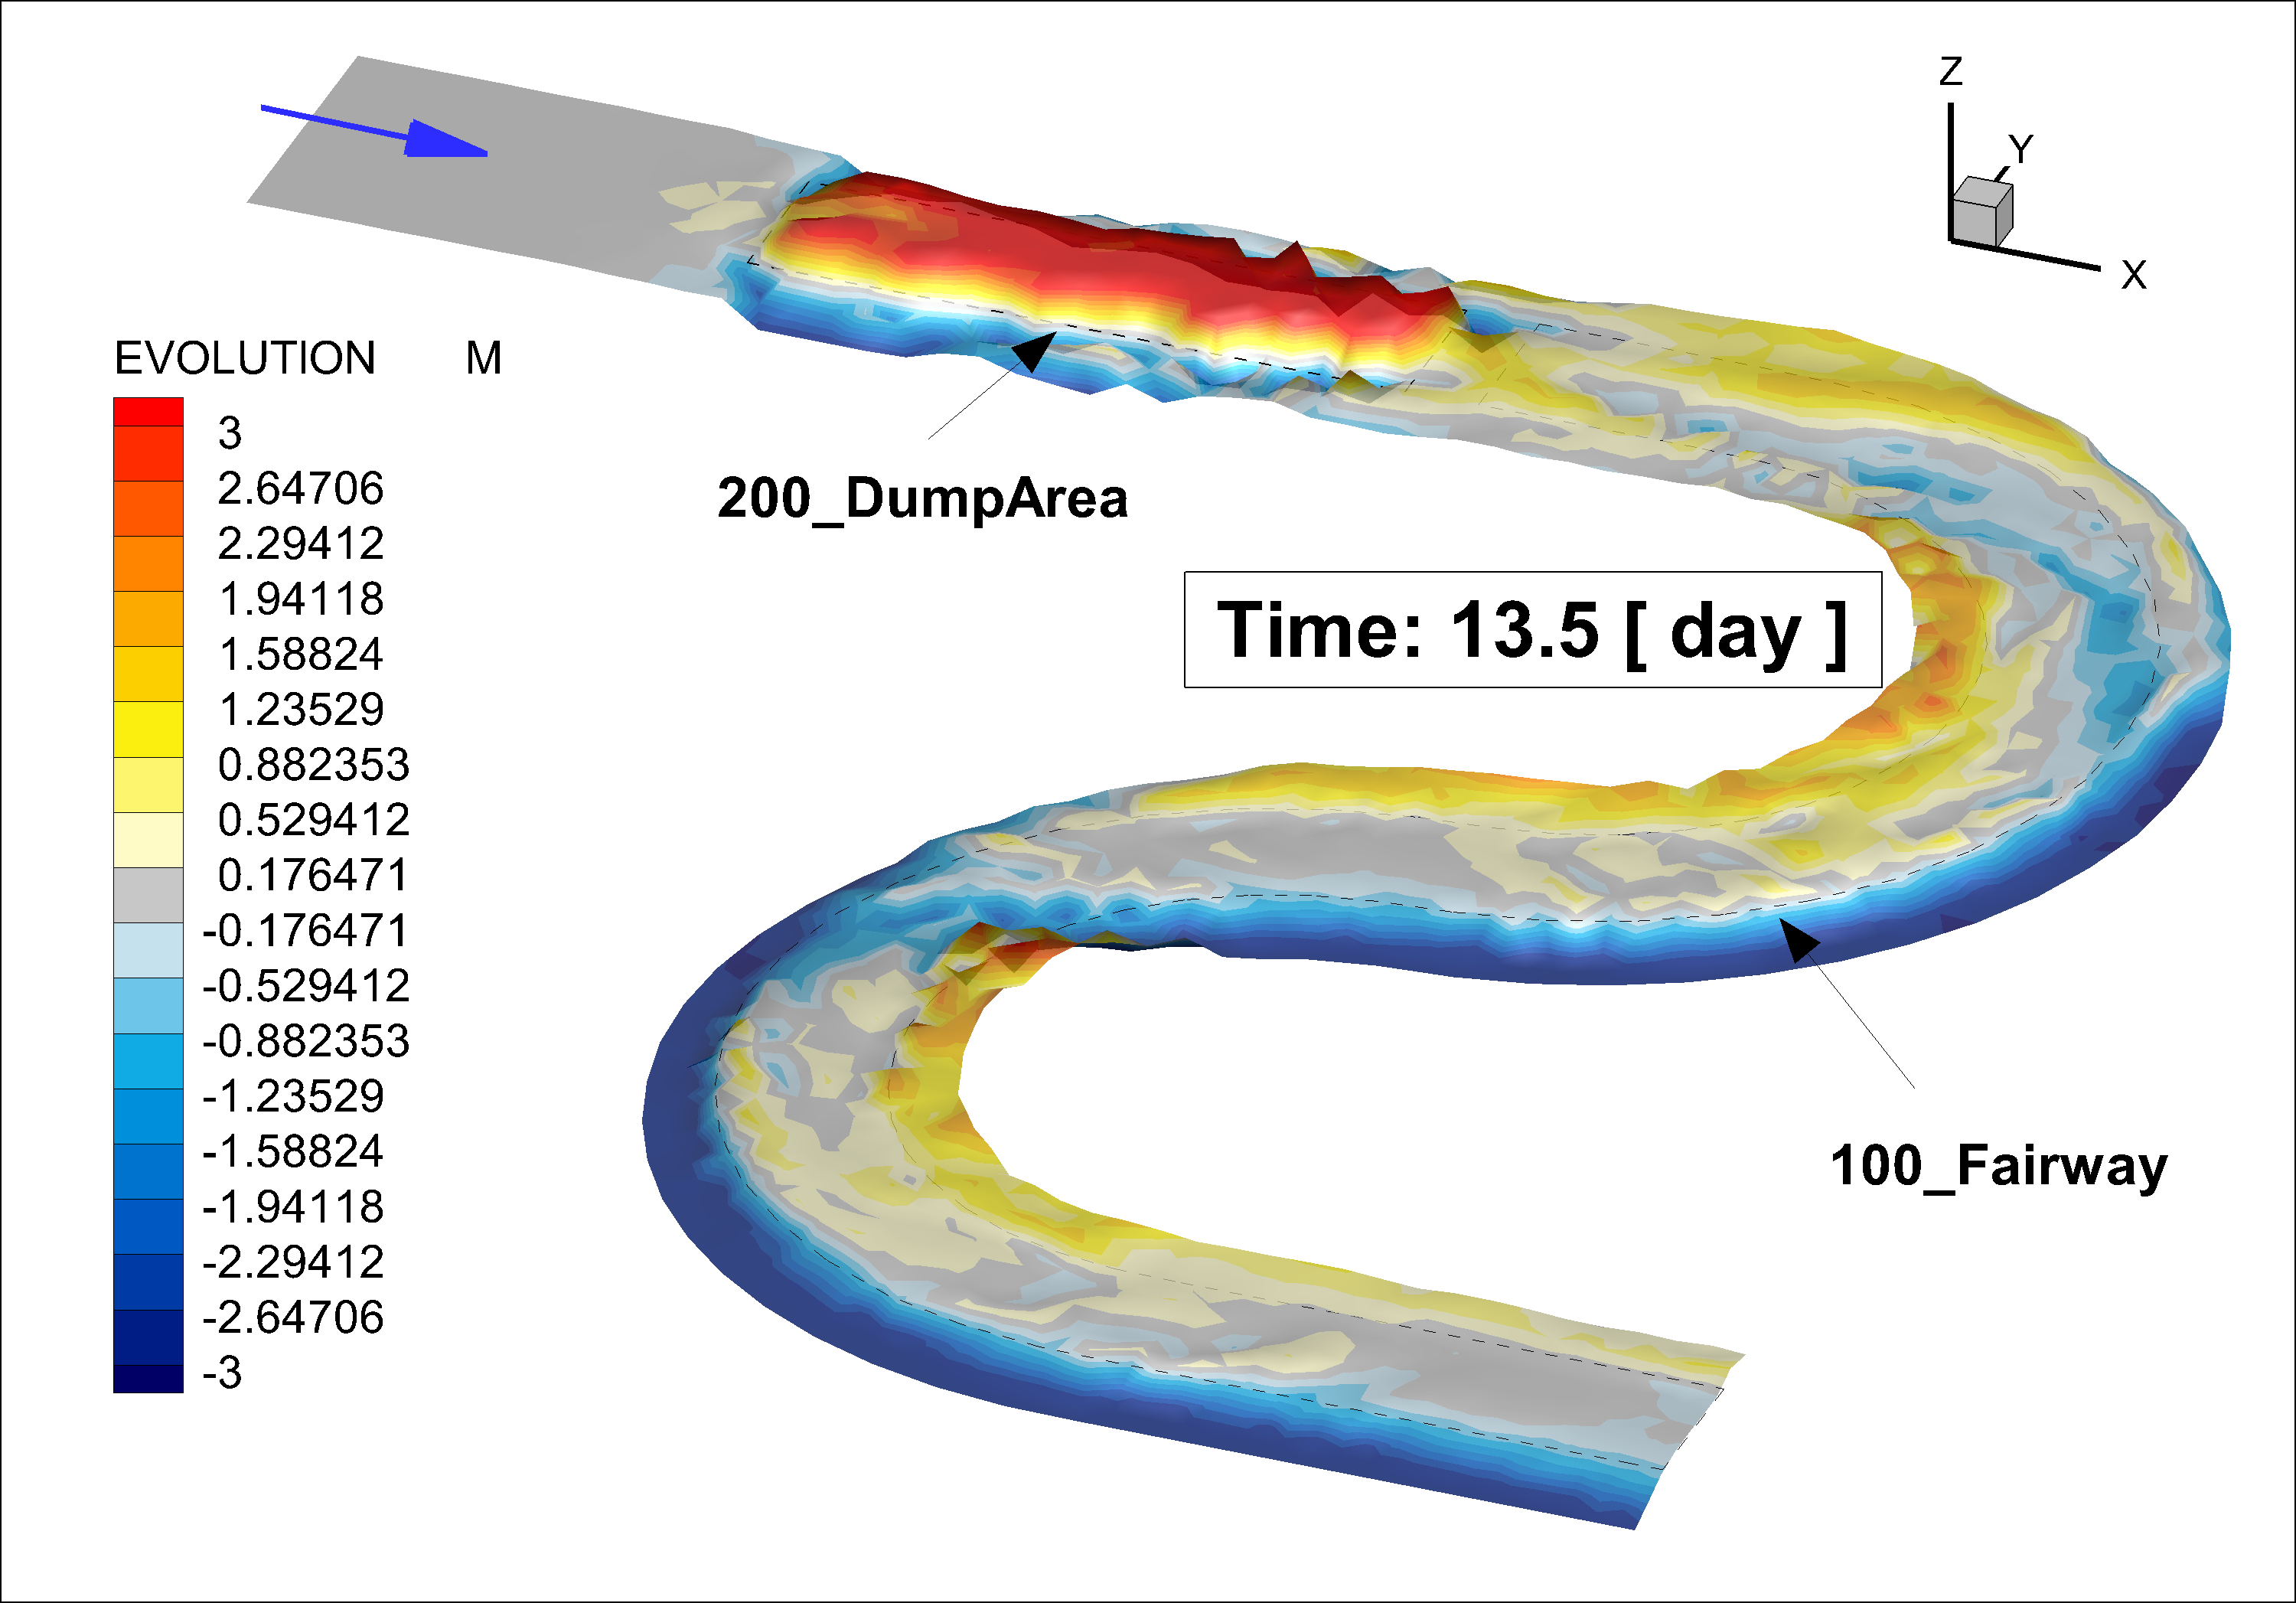
\includegraphics[scale=0.14]{critDig_Poly_13p5d.png}
\caption{Simulated evolution over the time.}\label{result78}
\end{figure}
